\documentclass[NewProceedings,letterpaper,NoPageNumbers,NoLineNumbers]{ascelike-new}
\WarningFilter{caption}{Unknown document class}
%% Please choose the appropriate document class option:
% "Journal" produces double-spaced manuscripts for ASCE journals.
% "NewProceedings" produces single-spaced manuscripts for ASCE conference proceedings.
% "Proceedings" produces older-style single-spaced manuscripts for ASCE conference proceedings. 
%
%% For more details and options, please see the notes in the ascelike-new.cls file.

% Some useful packages...
\usepackage[utf8]{inputenc}
\usepackage[T1]{fontenc}
\usepackage{lmodern}
\usepackage{graphicx}
\graphicspath{{../figures/}}
\usepackage[style=base,figurename=Fig.,labelfont=bf,labelsep=period]{caption}
\usepackage{subcaption}
\usepackage{amsmath}
\usepackage{newtxtext,newtxmath}
\usepackage[colorlinks=true,citecolor=red,linkcolor=black]{hyperref}
%
% Please add the first author's last name here for the footer:
% \NameTag{AuthorOneLastName, \today}
% Note that this is not displayed if the NoPageNumbers option is used
% in the documentclass declaration.
%
\begin{document}

% You will need to make the title all-caps
\title{Prediction of Building Component Condition Assessment Scores}

\author[1]{Eric Mixon}
\author[2]{Juliana Marks}
\author[3]{Julian Hwang}

\affil[1]{Email: ermixon2@illinois.edu}
\affil[2]{Email: jm128@illinois.edu}
\affil[3]{Email: jzhwang3@illinois.edu}
\maketitle

\section{Introduction}

Sustainment of very large real property portfolios requires many complex decisions. When a few decision makers must allocate constrained maintenance funding across millions of facilities, informed individual repair/replace decisions become infeasible for the whole portfolio. Real property managers in this situation rely on mathematical models to assist with funding distribution and work action decisions across the large scope.  These sustainment decision models generally rely on condition information about the inventory within the portfolio to drive their decision-making. This is known as a knowledge-based decision model.  In many cases, it is infeasible to install condition sensors on every component of every facility, so knowledge-based models will use expert observations in the form of condition assessments to inform inventory condition.  While sustainment models can attempt to predict condition deterioration over time, much like weather prediction models, they are only reliable for short-term horizons. So, periodic re-observations are required through assessment contracts with large A\&E firms to collect and update condition information.  

Stemming from these requirements comes a need for real property managers to decide what inventory in their portfolio is due for re-observation.  Historically, the most common method is to simply reassess everything every 5 years (i.e. 20\% of the portfolio per year).  To reduce the amount and therefore cost of these assessments, a value of information (VOI) strategy could be utilized to make informed selections of which assets or components within the inventory are of the highest value to re-assess (i.e. the most likely to improve our maintenance investment decisions).  A critical requirement of this model is to be able to predict what scores an assessor would likely assign to a component based on historical data. 

\subsection{Dataset}

The dataset used for this project comes from assessment data in the Sustainment Management System (SMS) BUILDER platform developed by Construction Engineering Research Laboratory (CERL). The full dataset includes approximately 2.7 million observations. Observations include both a manually collected direct condition rating and a predicted condition index generated from component information using the SMS Weibull degradation model at the time of an assessment. Multiple observations can be generated for given components if they have multiple assessment records. The observation's predicted CI (Condition Index) is generated using the following:

\begin{equation}
\label{eq:sms-weibull-ci}
\mathrm{CI}(t) = A \left( \frac{100}{\mathrm{CI}_{\mathrm{T}}} \right)^{ -\left(\frac{t}{\beta}\right)^{\alpha} }
\end{equation}

Where $\mathrm{t}$ is the normalized age of the component, $\mathrm{CI_T}$ is the design life of the component, A is the initial starting condition (usually 100), $\alpha$ is the scale or characteristic age of replacement, and $\beta$ is the shape or degradation parameter. The $\alpha$ and $\beta$ parameters are provided from a per specification reference catalog within the SMS, however these values can be shifted after assessments to adjust the curve to fit to the assessed condition. In cases where components have multiple assessments, observations use the SMS $\alpha$ and $\beta$ shift calculations prior to calculating the predicted CI; this ensures continuity with the prediction at the time of the assessment. A detailed intuition for the Weibull model is available using the Desmos tool that can be found at \url{https://www.desmos.com/calculator/cenbpl3qtf}. The final resulting observations also capture other information about the component. See Table~\ref{table:assembly} for complete details.

Assessment scores generally are collected as "Direct Condition Ratings", amounting to a selection from 9 possible score options. An example criterion for these scores can be found below in Table \ref{table:AssessmentScores} (Not all organizations have exactly the same criterion, but the score choices are always the same). Most organizations have additional guidance through large (sometimes 1000's of pages) assessment guides. These guides direct the types of components to inventory and assess, when and how to input comments about the assessment, additional criterion for scoring for specific component types, and other data quality governance. 

\subsection{Proposed Objectives}

Although the dataset consists of 2.7 million observations, a subset corresponding to a single material equipment category (MEC) will be used for this project. The MEC for boilers consists of 12,832 assessments, so it should be possible to perform a detailed analysis for the specifications within this MEC. The goal of this study will be to identify the best parameters about a component that would inform the best possible predictions about a likely assessment score distribution.  The study could also explore different types of models such as binning solutions, decision trees (XGBoost), ANNs, or other class-based solutions to find which of the options would inform the best predictions.

The proposed workflow for the project is:
\begin{enumerate}
\item Perform initial exploratory analysis to identify data wrangling needs and potential data bias.
\item Perform Principal Component Analysis (PCA) to identify the best predictive parameters.
\item Build a prediction model returning multi-class distribution using a Artificial Neural Network (ANN) trained on identified principal components.
\item Build a prediction model returning multi-class distribution using XGBoost (or other decision tree library) trained on identified principal components.
\item Build additional prediction models based on in-class statistical learning solutions.
\item Perform comparative study between prediction models to identify which has the best predictive performance.
\end{enumerate}

\newpage

\section{Exploratory Data Analysis}

\subsection{Basic Data Description and Initial Questions}

The first steps of data exploration began with simply visualizing the shapes of individual columns of the dataset to get a feel for the distributions of the data. Distributions were produced and explored for all fields, but only a few are highlighted for focus on observations that motivated the questions that followed. The first two major columns include the predicted condition score or Condition Index (CI) of the weibull degradation model and the actual observed score of the assessor (i.e. The assessor rating).  Immediately there is an identifiable difference between the expected degradation and the assessed scores (Figures \ref{fig:ci_dist} and \ref{fig:score_dist}).  There also seems to be a heavy bias toward ratings of 88 in the observations.

There are some rational narratives that can explain the disagreement in predicted and assessed scores.  The SMS system from which the observations are sourced is used by organizations to plan maintenance management.  Work analysis rules are put into place within the system to prioritize maintenance funding allocation.  For "D30" systems (mechanical systems in UNIFORMAT which includes boilers), a typical ruleset will specify that components with CI less than 85 should be marked for repair action, and components with a remaining service life (RSL) of less than 2 should be marked for replacement. If maintenance dollars are being executed by that guidance, then it would be expected that assessors rarely come across boilers with condition less than 85.  This also makes rational sense from a facility function perspective, HVAC systems tend to get immediate attention when they fail, as they are considered critical for most facilities. A score of 88 represents a well maintained and functioning unit, which is what is expected based on maintenance priority. Additionally, this bias is not unique to SMS data, and has been observed in other inspection/assessment based condition datasets. One such example is an Ontario bridge inspection dataset where a similar condition clustering is observed at around 77 (Based on their unique condition rating system) \cite{ontario_bridge_conditions_2021}.

Based on this visual inspection of the assessed score distribution.  Questions were formulated to attempt to identify how data could potentially be classified in a way that distinguishes between the boilers that are kept to specified condition, and the ones that are allowed to deteriorate. Answering this question can potentially improve the feature selection for a prediction model. Looking at few of the other distributions including RSL(Figure \ref{fig:rsl_dist}), Month(Figure \ref{fig:month_dist}), Climate(Figure \ref{fig:climate_dist}) raised possible considerations which included hypothesis such as:

\begin{itemize}
    \item Does RSL (or other lifecycle variables) correlate with assessor ratings?
    \item Does the month (i.e Season) of the assessment impact the expected assessed condition for boilers?
    \item Does the climate (warm or cold) impact expected assessed condition? (Note: Figure \ref{fig:doe_climate_map} illustrates the climate zones used in the observations)
    \item Do specific facility types show maintenance priority?
    \item What other ways could the data be classified to help with prediction models?
\end{itemize}

\begin{figure}
\centering
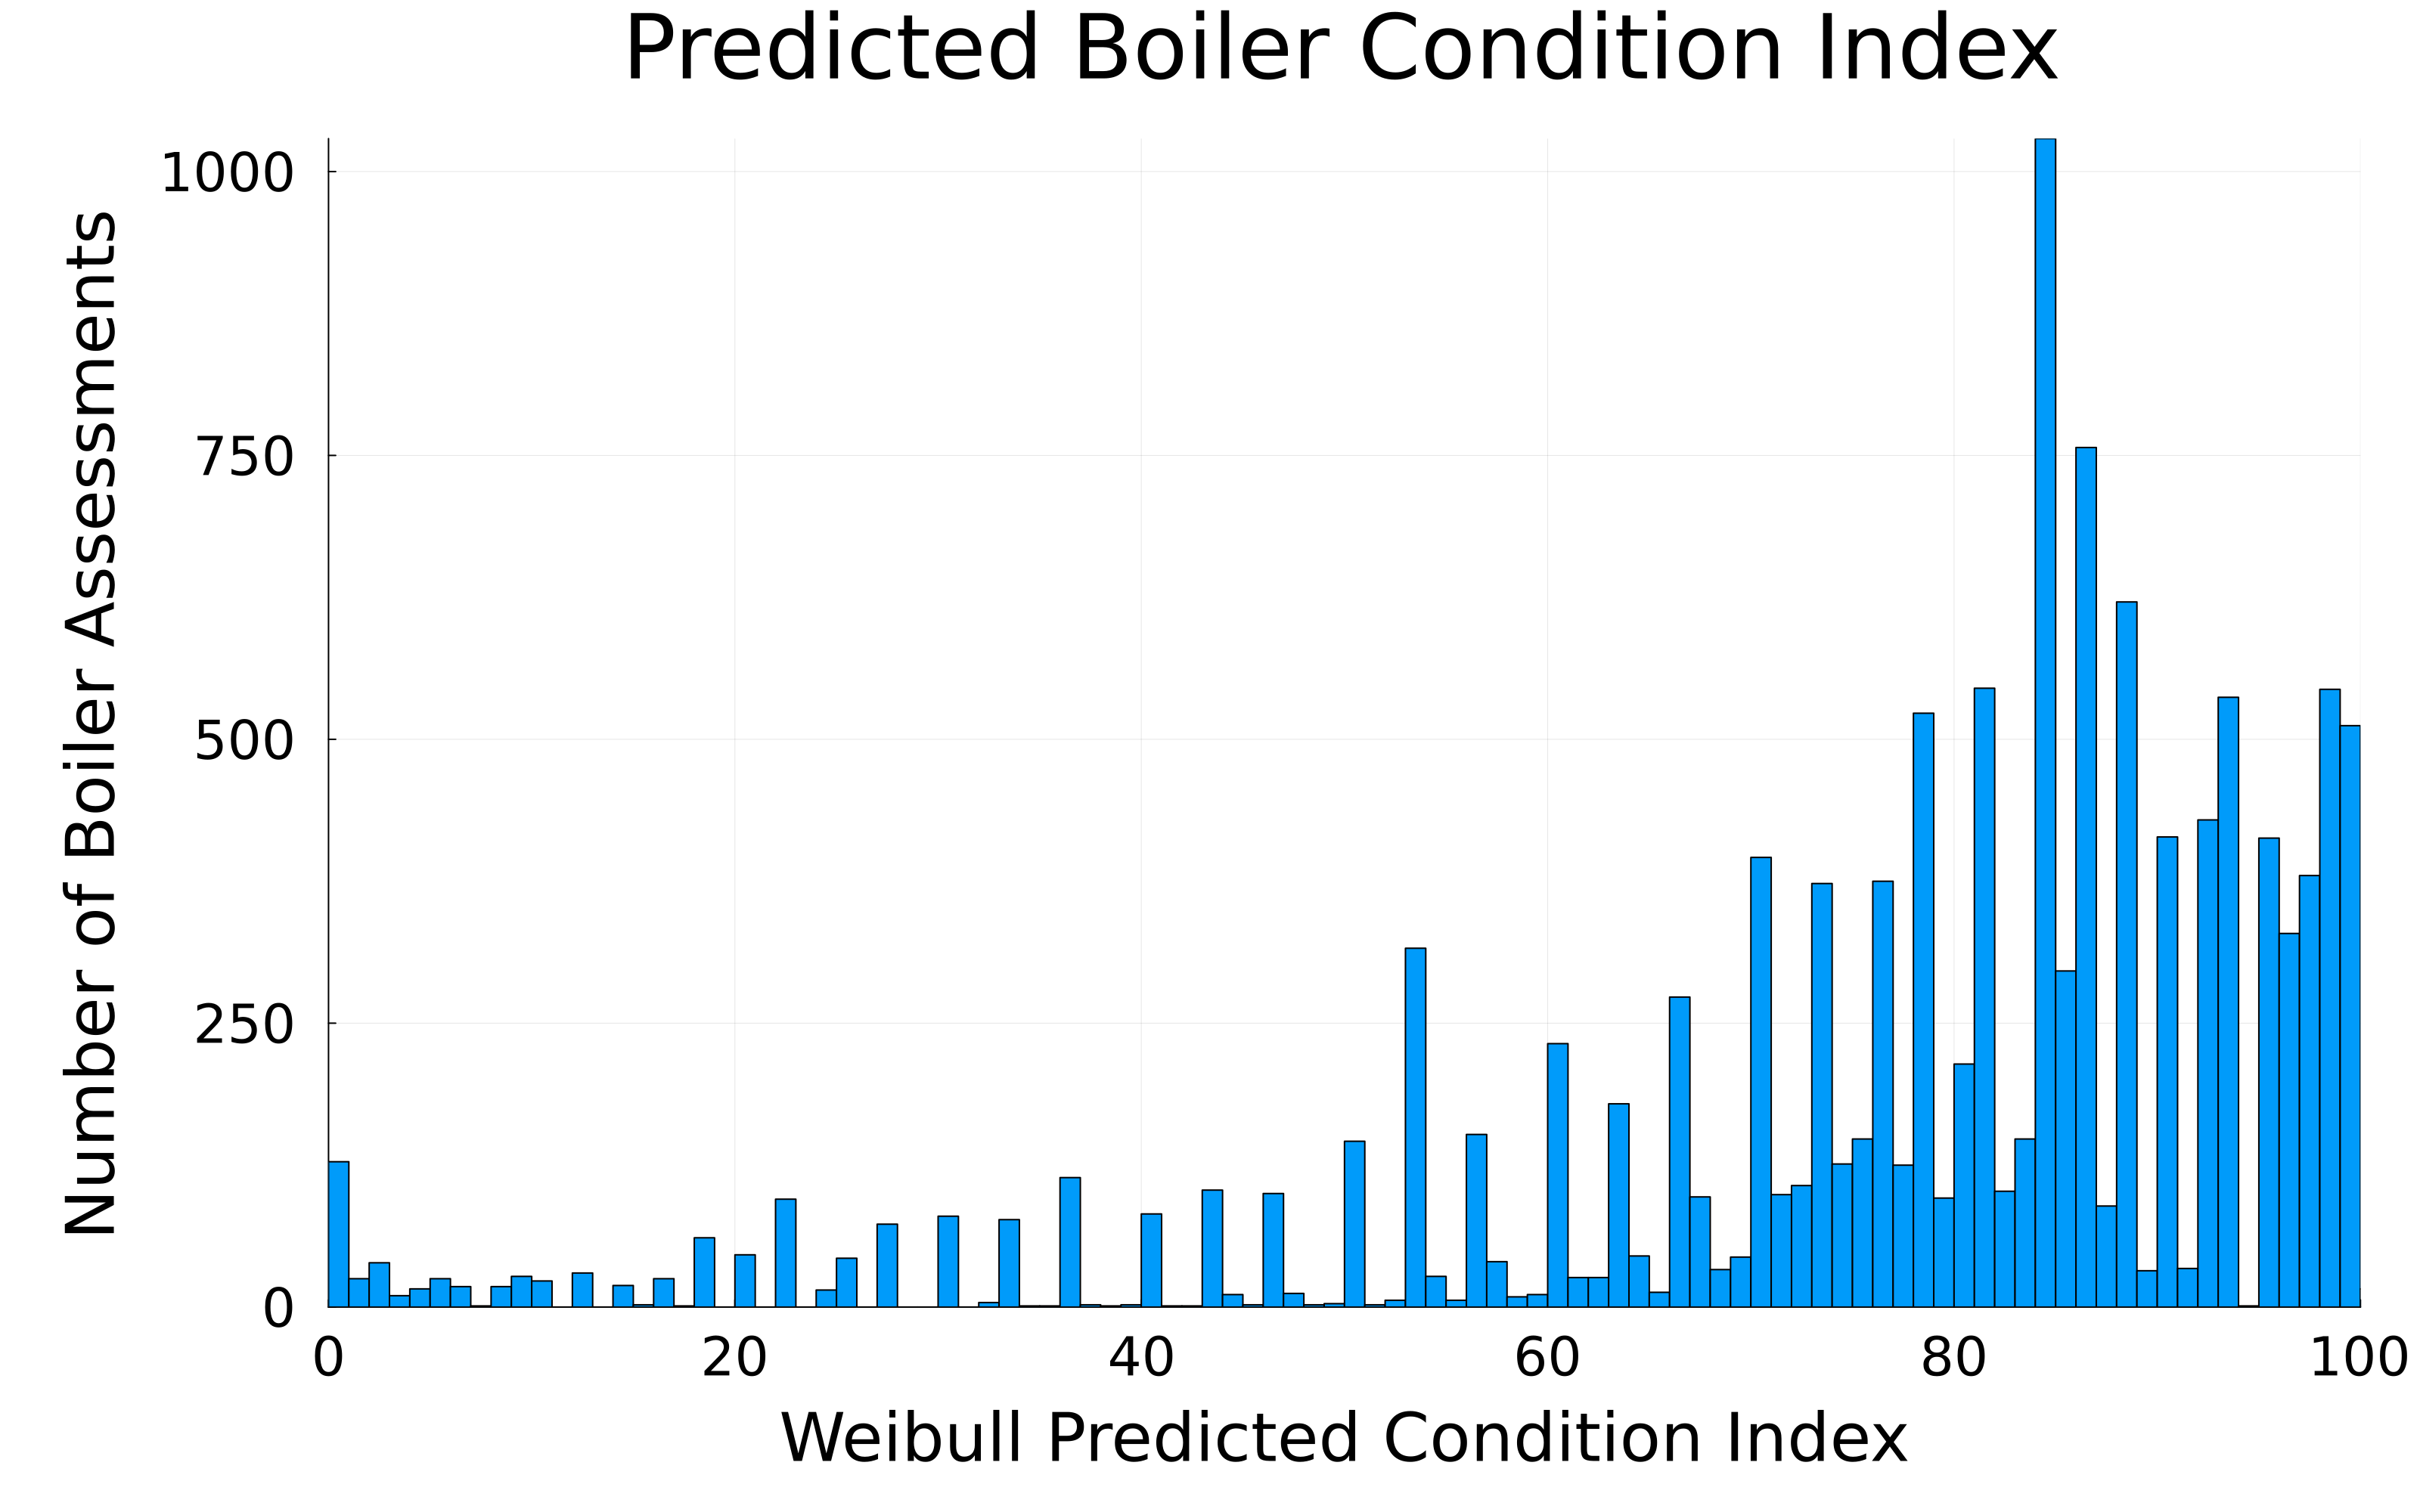
\includegraphics[width=1\linewidth]{ci_dist.png}
\caption{Predicted CI Distribution}
\label{fig:ci_dist}
\end{figure}

\begin{figure}
\centering
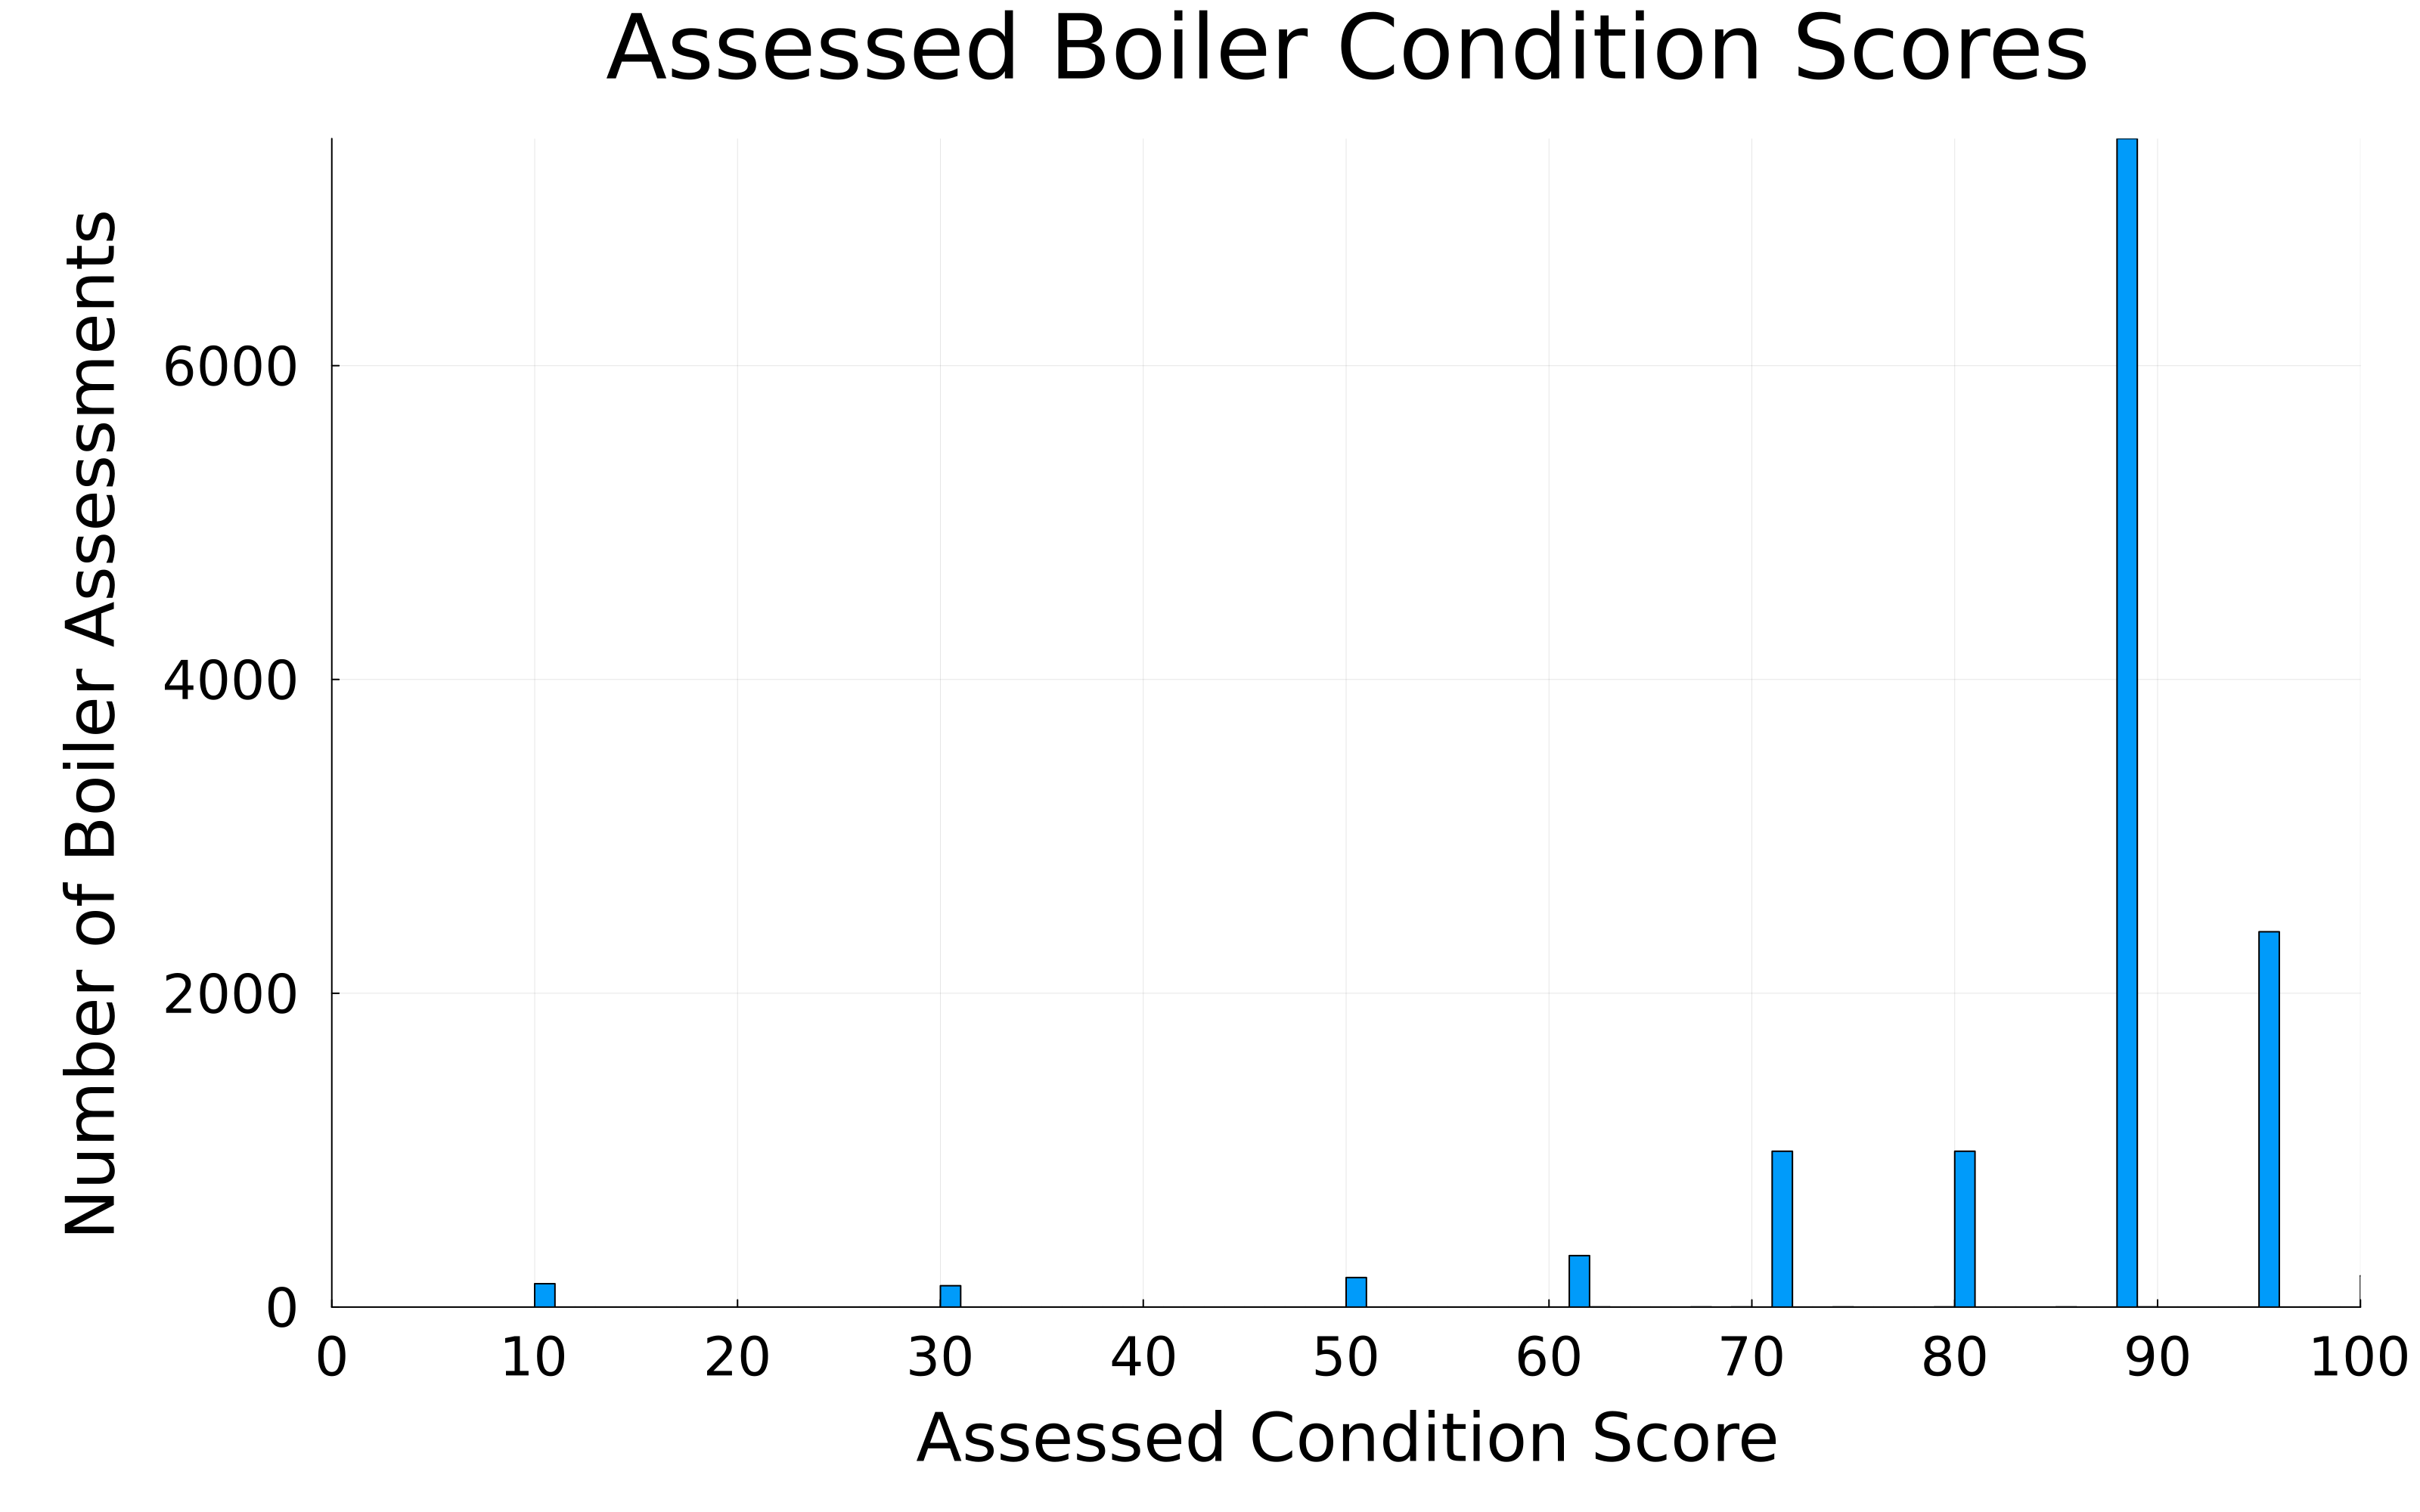
\includegraphics[width=1\linewidth]{score_dist.png}
\caption{Assessment Score Distribution}
\label{fig:score_dist}
\end{figure}

\begin{figure}
\centering
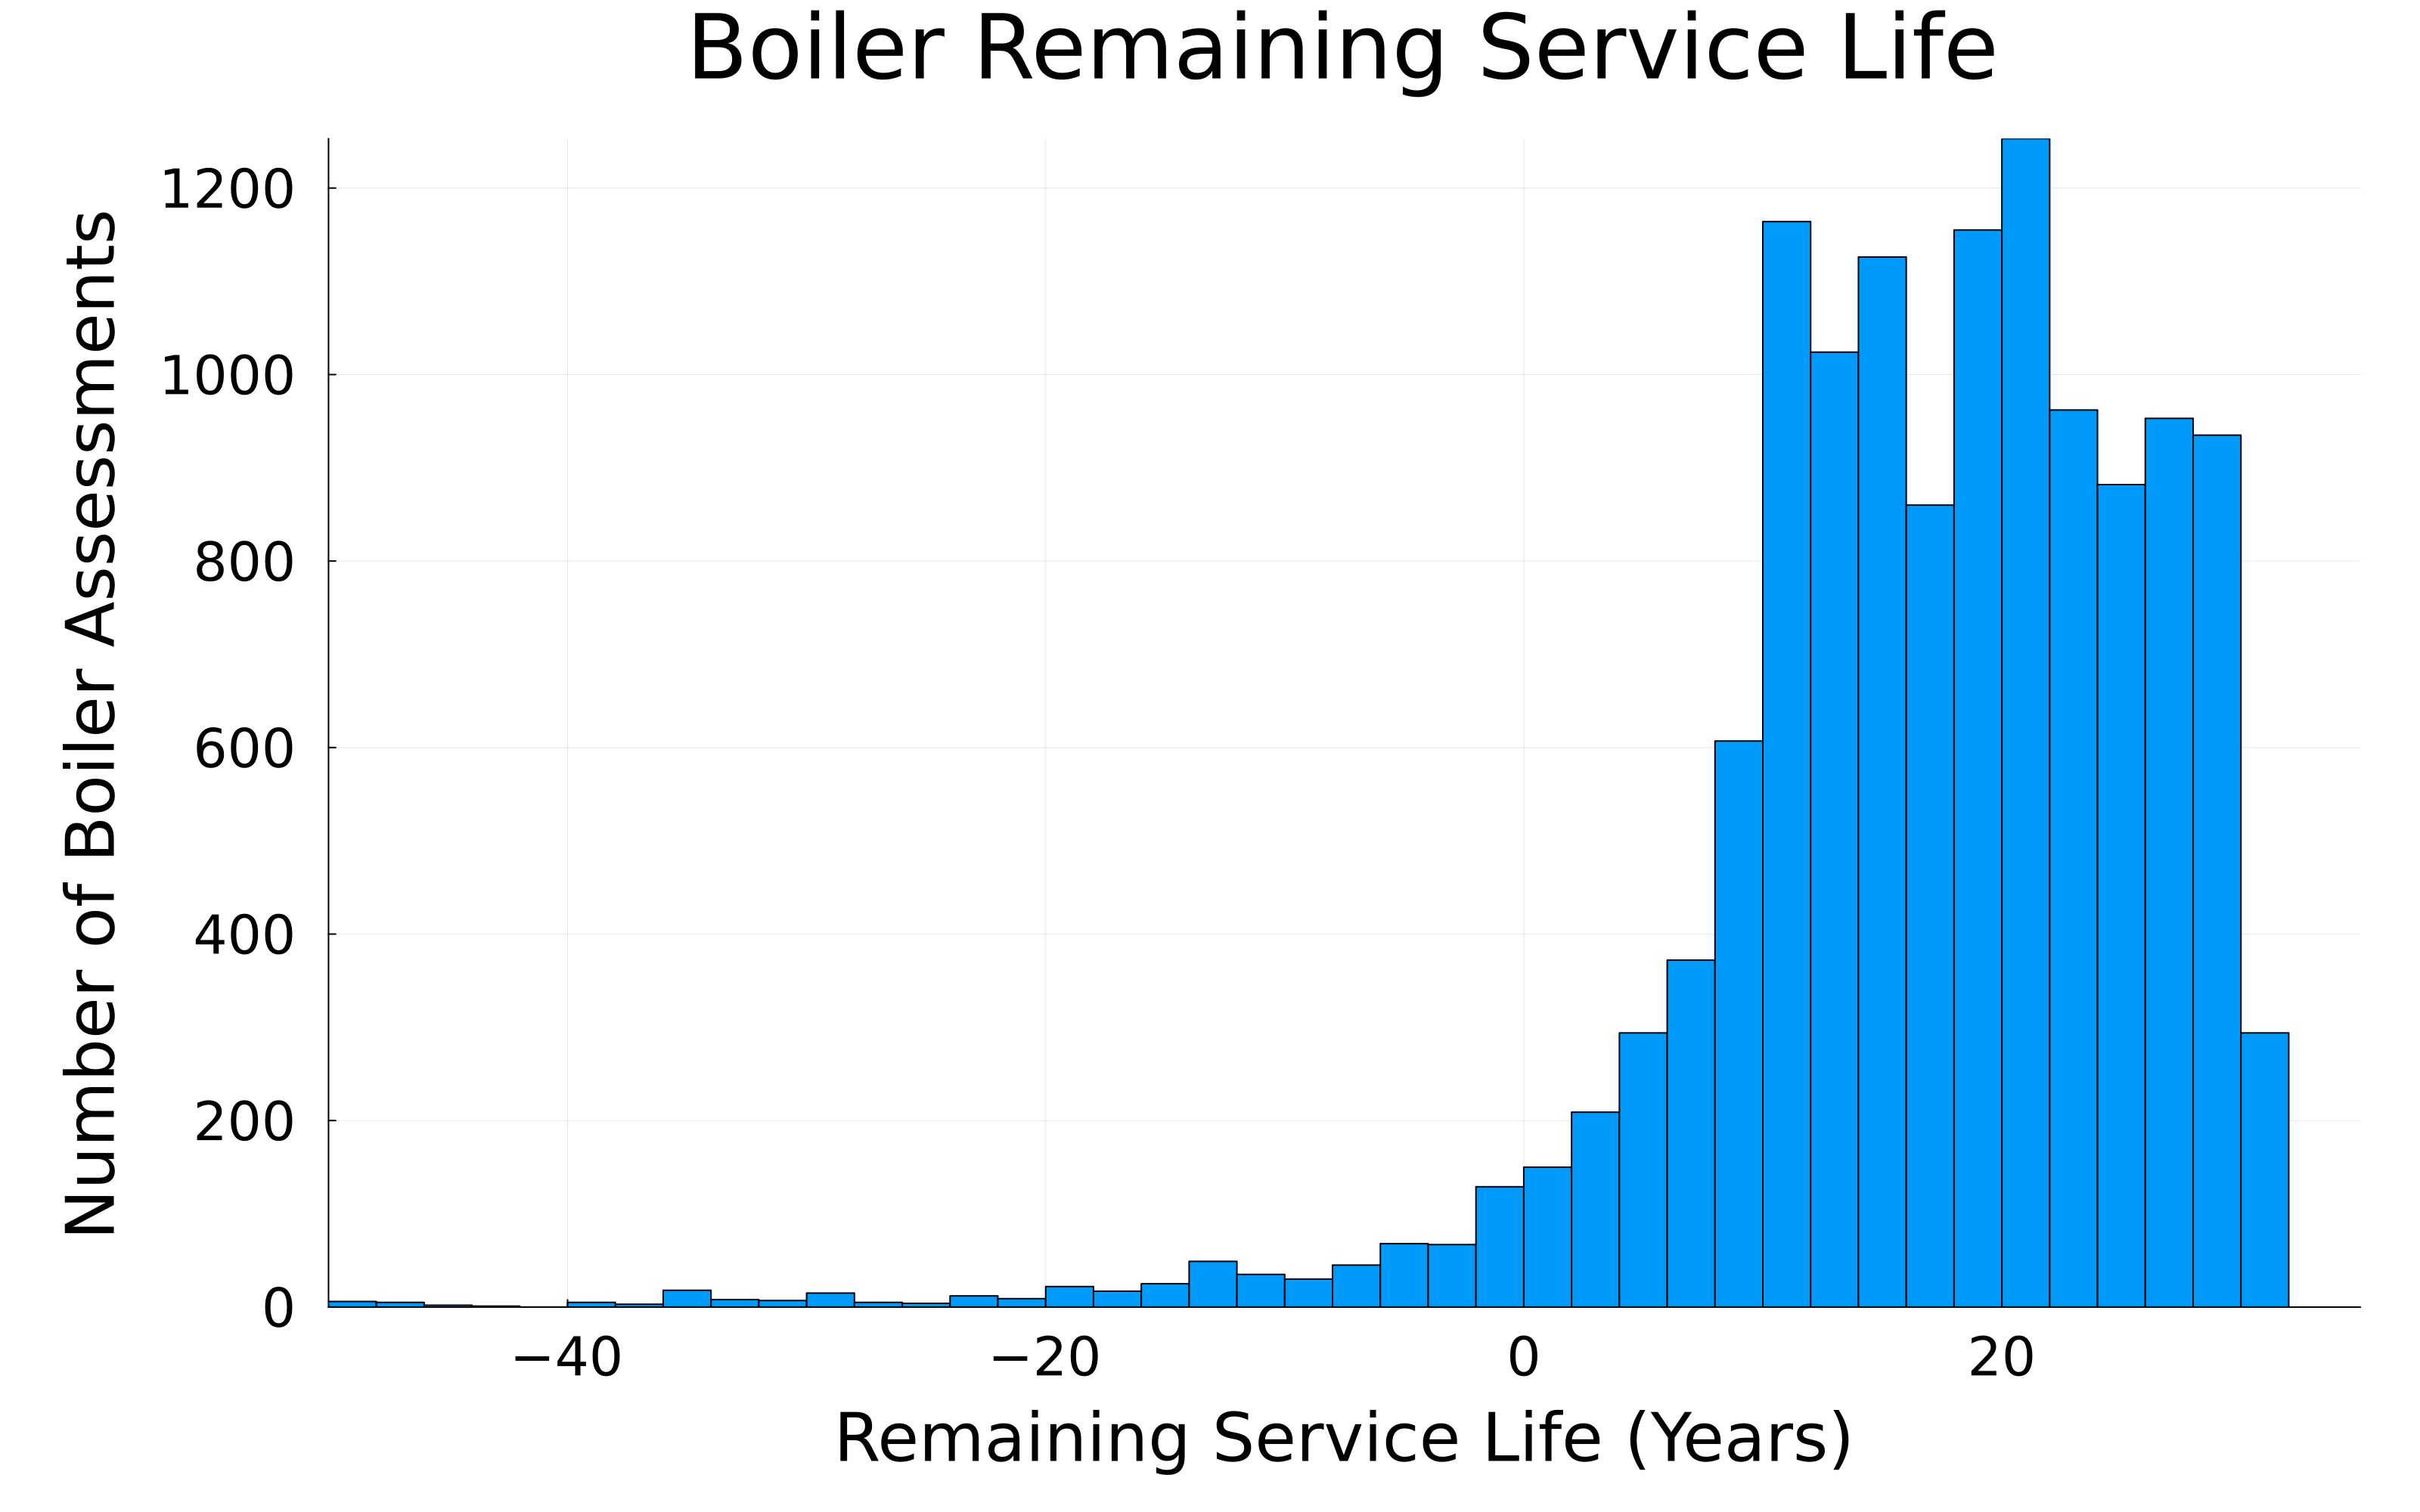
\includegraphics[width=1\linewidth]{rsl_dist.png}
\caption{Remaining Service Life Distribution}
\label{fig:rsl_dist}
\end{figure}

\begin{figure}
\centering
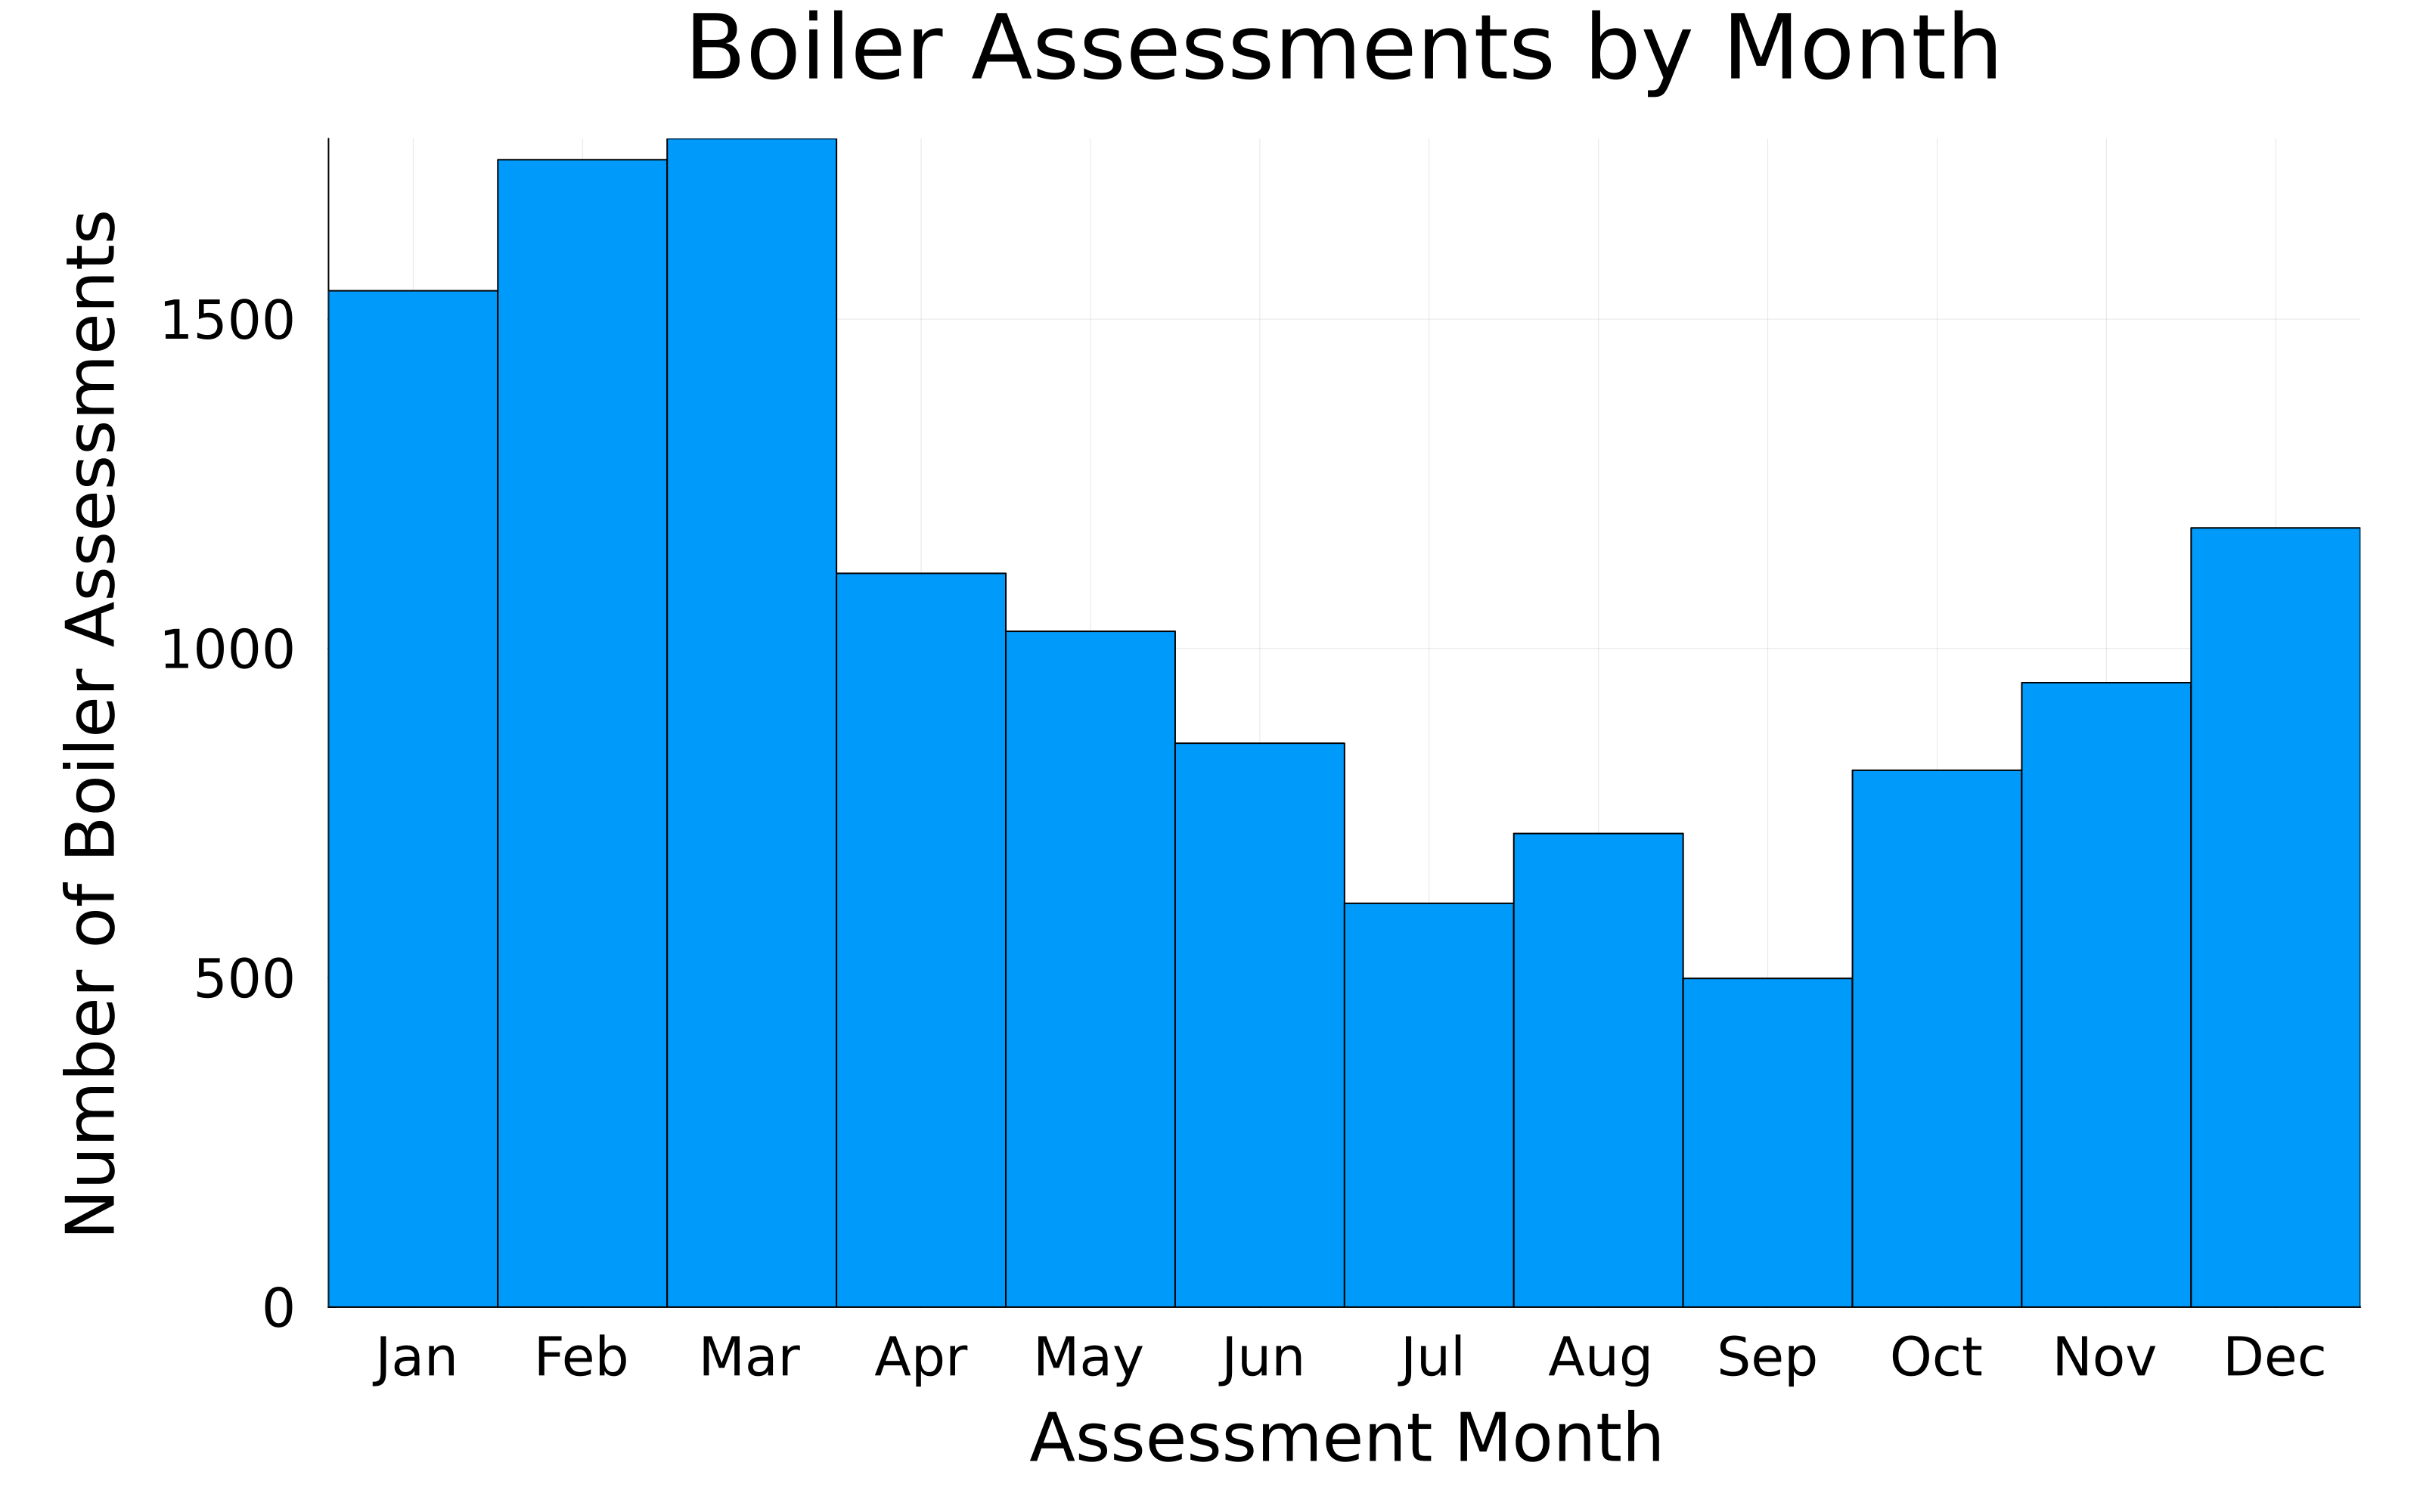
\includegraphics[width=1\linewidth]{month_dist.png}
\caption{Assessment Month Distribution}
\label{fig:month_dist}
\end{figure}

\begin{figure}
\centering
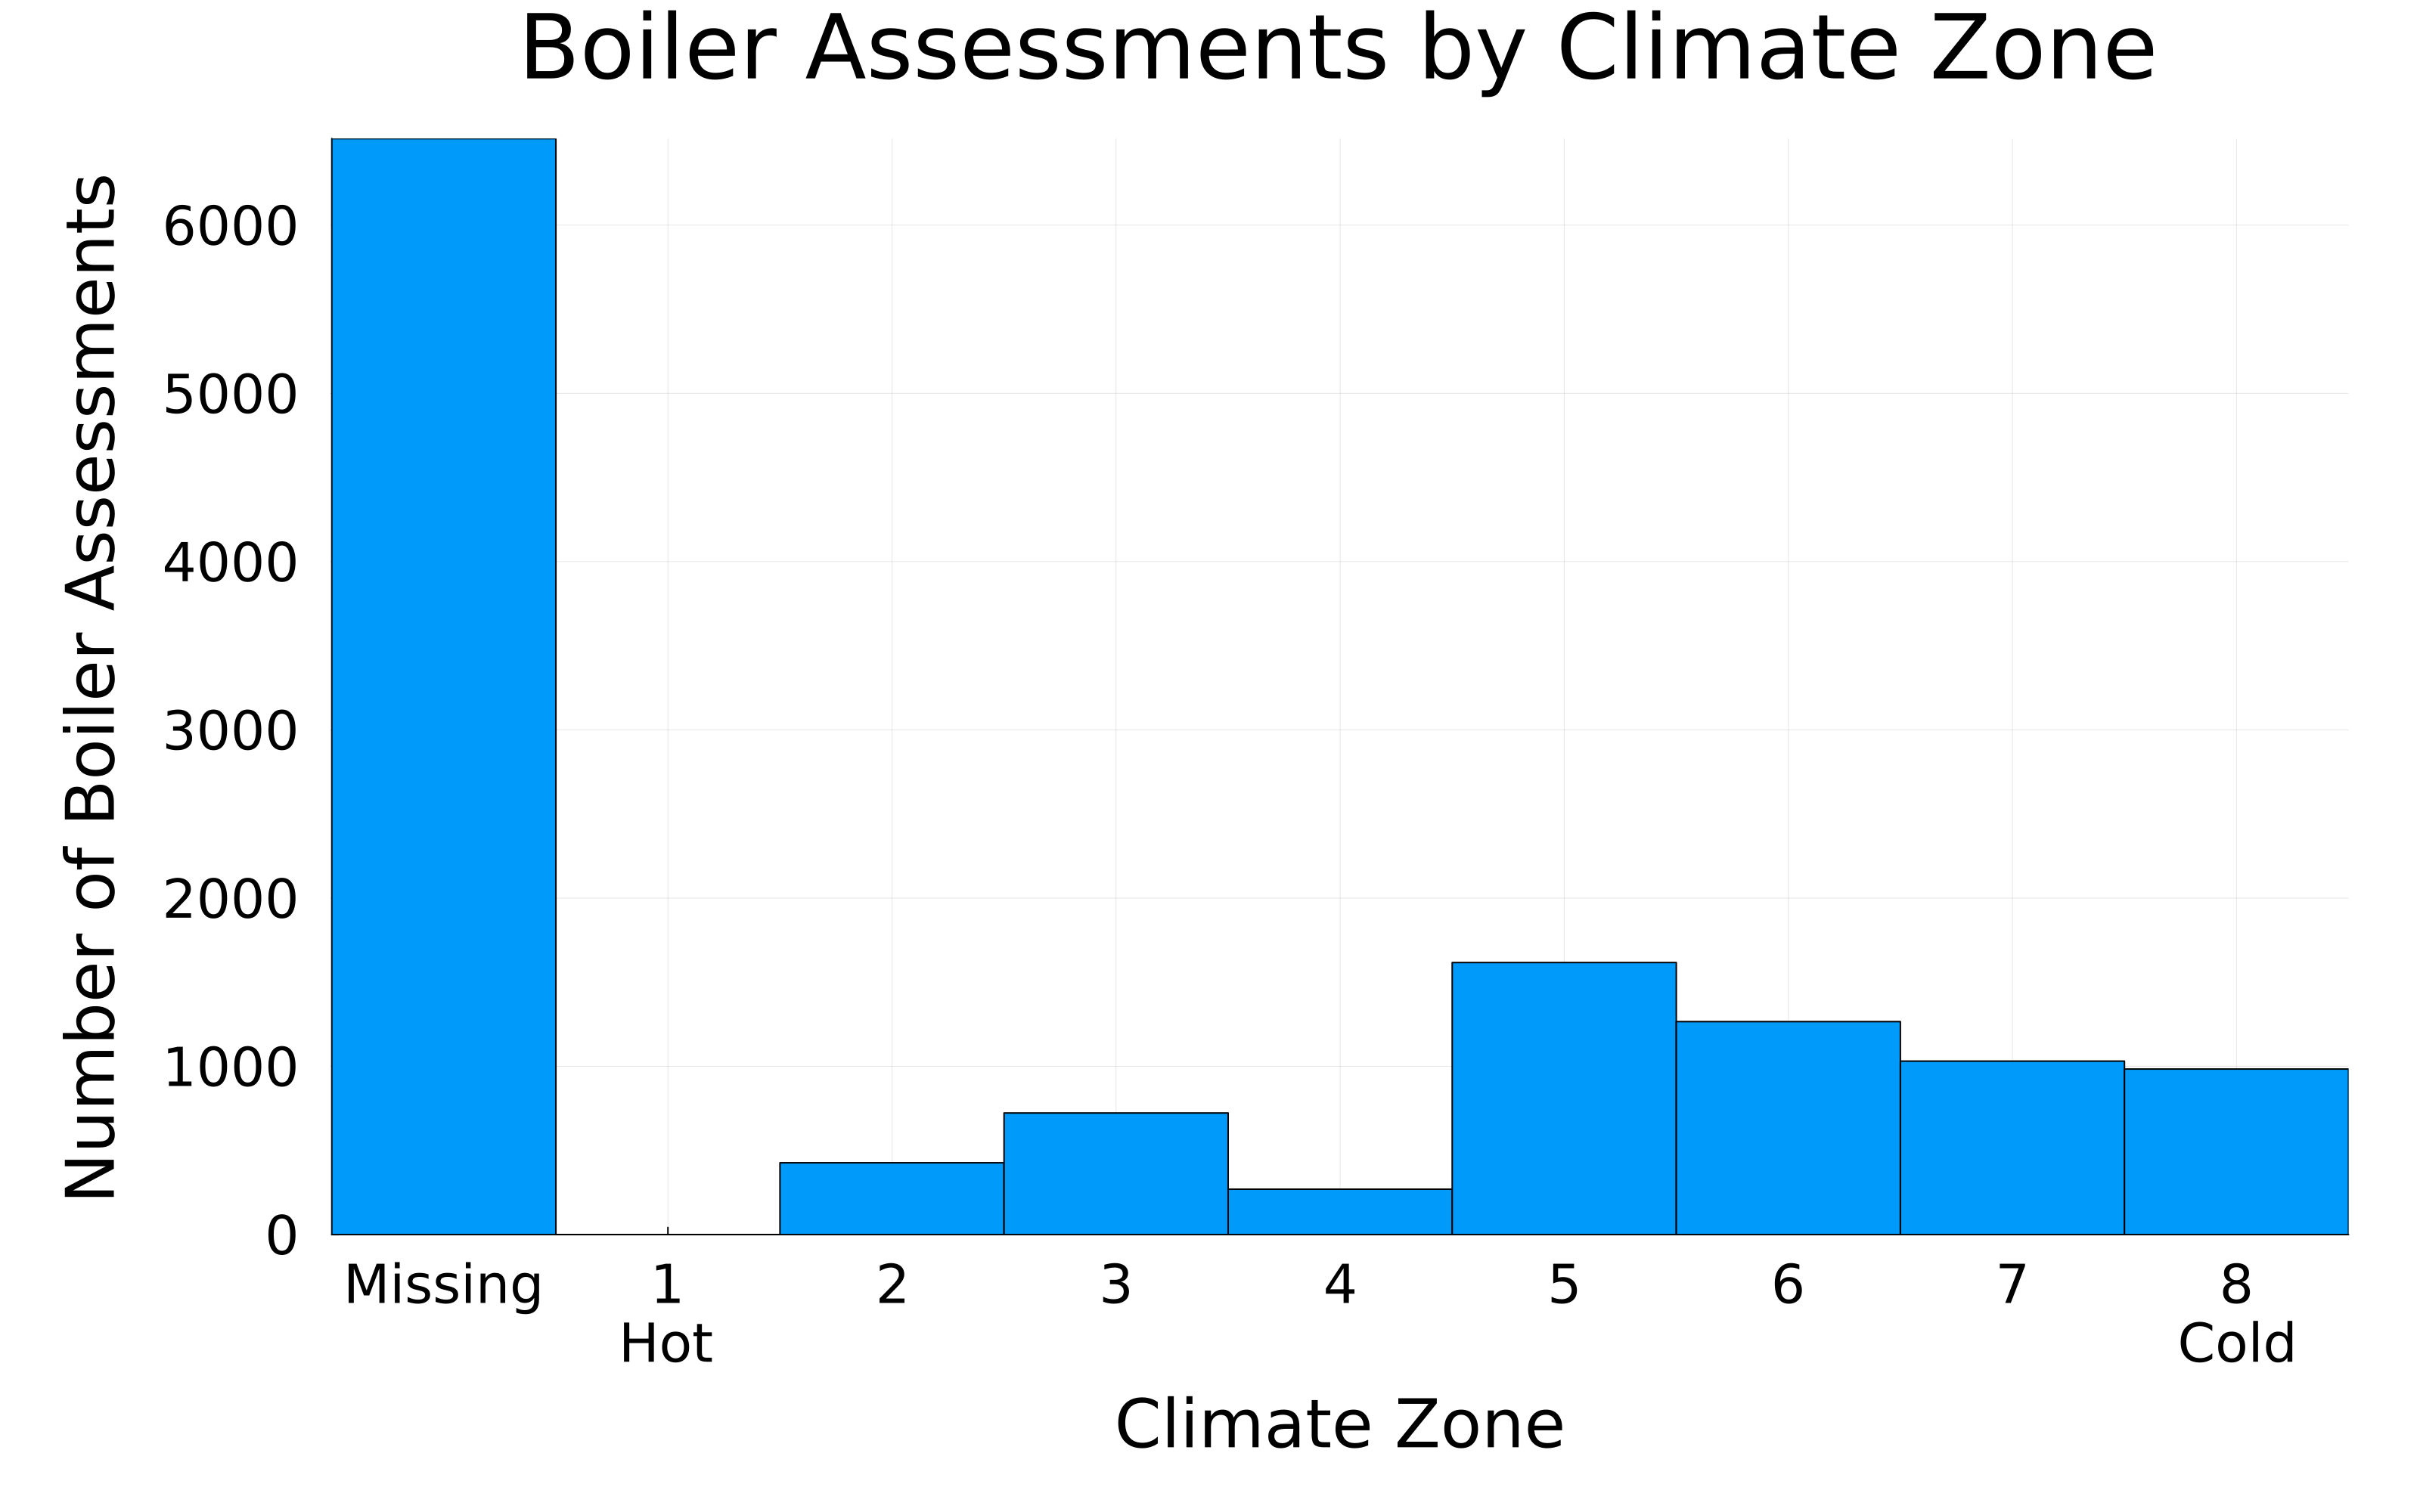
\includegraphics[width=1\linewidth]{climate_dist.png}
\caption{Assessment Climate Distribution}
\label{fig:climate_dist}
\end{figure}

\begin{figure}
\centering
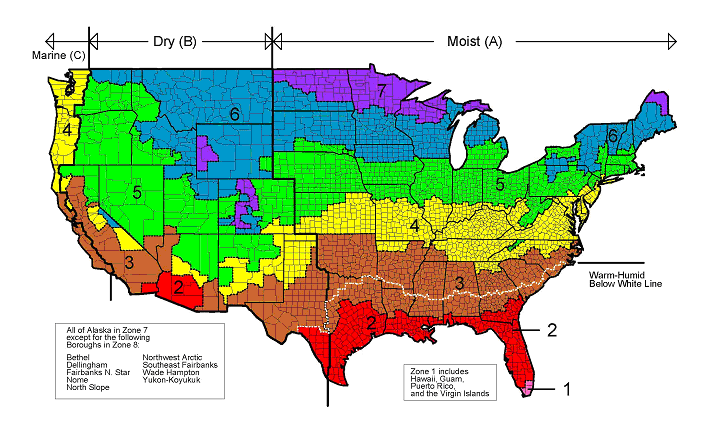
\includegraphics[width=1\linewidth]{DOE_Climate_Zones.png}
\caption{Dept. of Energy Climate Zones Map \protect\cite{doe_building_america_climate_guidance}}
\label{fig:doe_climate_map}
\end{figure}

\newpage

\subsection{Pre-PCA Data Wrangling}

Before a Principal Component Analysis (PCA) could be performed, the data needed a bit of cleaning.  Table \ref{tab:boiler_descriptive_statistics} shows some basic statistics of the raw dataset. Notice that some columns such as Recency, Climate, and PrevScore have missing values. Additionally, some columns represent non-ordinal identifiers that are not typically useful in PCA and most of the ordinal columns are in mixed types and ranges varying by several orders of magnitude. To address these issues, a number of data wrangling steps are performed:

\begin{enumerate}
    \item For Recency and PrevScore, the missing data here represents components that have never previously been assessed. Since "Never Assessed" is potentially a valuable data point, the first step is to create a new column called "PrevAssessed" which will be 0 or 1 representing components that have or have not been assessed before.  Once the new column is created, missing values are replaced with the mean of available data in both Recency and PrevScore respectively.
    \item For Climate, the missing data here is simply missing data. Prior to PCA, the missing fields are populated with the mean of the known climate data.
    \item AssetAge and AssetDesignLife are better represented as a single property similar to the component NormalizedAge.  A new column is created called NormalizedAssetAge set to AssetAge / AssetDesignLife.
    \item For Month, since we are interested in impact of seasons on assessment scores, it is better to represent this data in a way that keeps the cyclical nature of seasons intact. Two new columns are created (MonthSin and MonthCos) representing the Month in a circular projection and keeping months like December and January close together ordinally.
    \item Component Replacement Value (CRV) is problematic in that is several orders of magnitude more than our other data fields.  Even with standardization of data prior to PCA, it may still be ordinally dominating. To address this, a new column is created called LogCRV representing the log of the original CRV values.  This brings the scale to a more comparable space and also makes a more symmetric dataset as can be seen in Figure \ref{fig:crv_log}
    \item Id, Spec, System, MEC, UOM, Fac, Qty, DesignLife, Month, AssetAge, and AssetDesignLife are omitted from the PCA analysis due to either being non-ordinal identifier columns, having the same value across nearly all the dataset (Qty, DesignLife), or having alternative suitable representations from the above wrangling steps.  Score is also omitted in the interest of avoiding data leakage when back loading for analysis potential predictive features. 
\end{enumerate}

\begin{table}[htbp]
\caption{Descriptive Statistics for Boiler Assessment Dataset Variables}
\label{tab:boiler_descriptive_statistics}
\centering
\small
\renewcommand{\arraystretch}{1.15}
\begin{tabular}{l r r r r r}
\hline\hline
\multicolumn{1}{c}{Variable} &
\multicolumn{1}{c}{Mean} &
\multicolumn{1}{c}{Minimum} &
\multicolumn{1}{c}{Maximum} &
\multicolumn{1}{c}{Missing} &
\multicolumn{1}{c}{Unique Values} \\
\hline
Id                & 4,673.27 & 1     & 9,334   & 0     & 9,334 \\
Spec              & 55.97    & 1     & 110     & 0     & 110 \\
System            & 1.00     & 1     & 1       & 0     & 1 \\
MEC               & 1.00     & 1     & 1       & 0     & 1 \\
DesignLife        & 30.00    & 15    & 30      & 0     & 2 \\
Qty               & 1.01     & 1     & 6       & 0     & 5 \\
UOM               & --       & Each  & Each    & 0     & 1 \\
Year              & 2020.91  & 2011  & 2025    & 0     & 15 \\
Month             & 5.64     & 1     & 12      & 0     & 12 \\
NormalizedAge     & 0.42     & 0.00  & 4.00    & 0     & 85 \\
EffectiveAge      & 16.72    & 0.00  & 121.00  & 0     & 84 \\
RSL               & 16.47    & -90.00& 30.00   & 0     & 278 \\
Recency           & 3.53     & 0.00  & 10.00   & 9,334 & 10 \\
Climate           & 5.52     & 2     & 8       & 6,514 & 7 \\
PredictedCI       & 76.48    & 0.00  & 100.00  & 0     & 435 \\
Score             & 84.78    & 10    & 100     & 0     & 16 \\
CRV               & 81,294.00& 6,290 & 902,540 & 0     & 965 \\
Fac               & 71.86    & 1     & 134     & 0     & 134 \\
AssetAge          & 38.75    & 0     & 181     & 0     & 154 \\
AssetDesignLife   & 51.12    & 30    & 60      & 0     & 11 \\
PrevScore         & 85.82    & 10    & 100     & 9,334 & 14 \\
\hline\hline
\end{tabular}
\end{table}

\begin{figure}
\centering
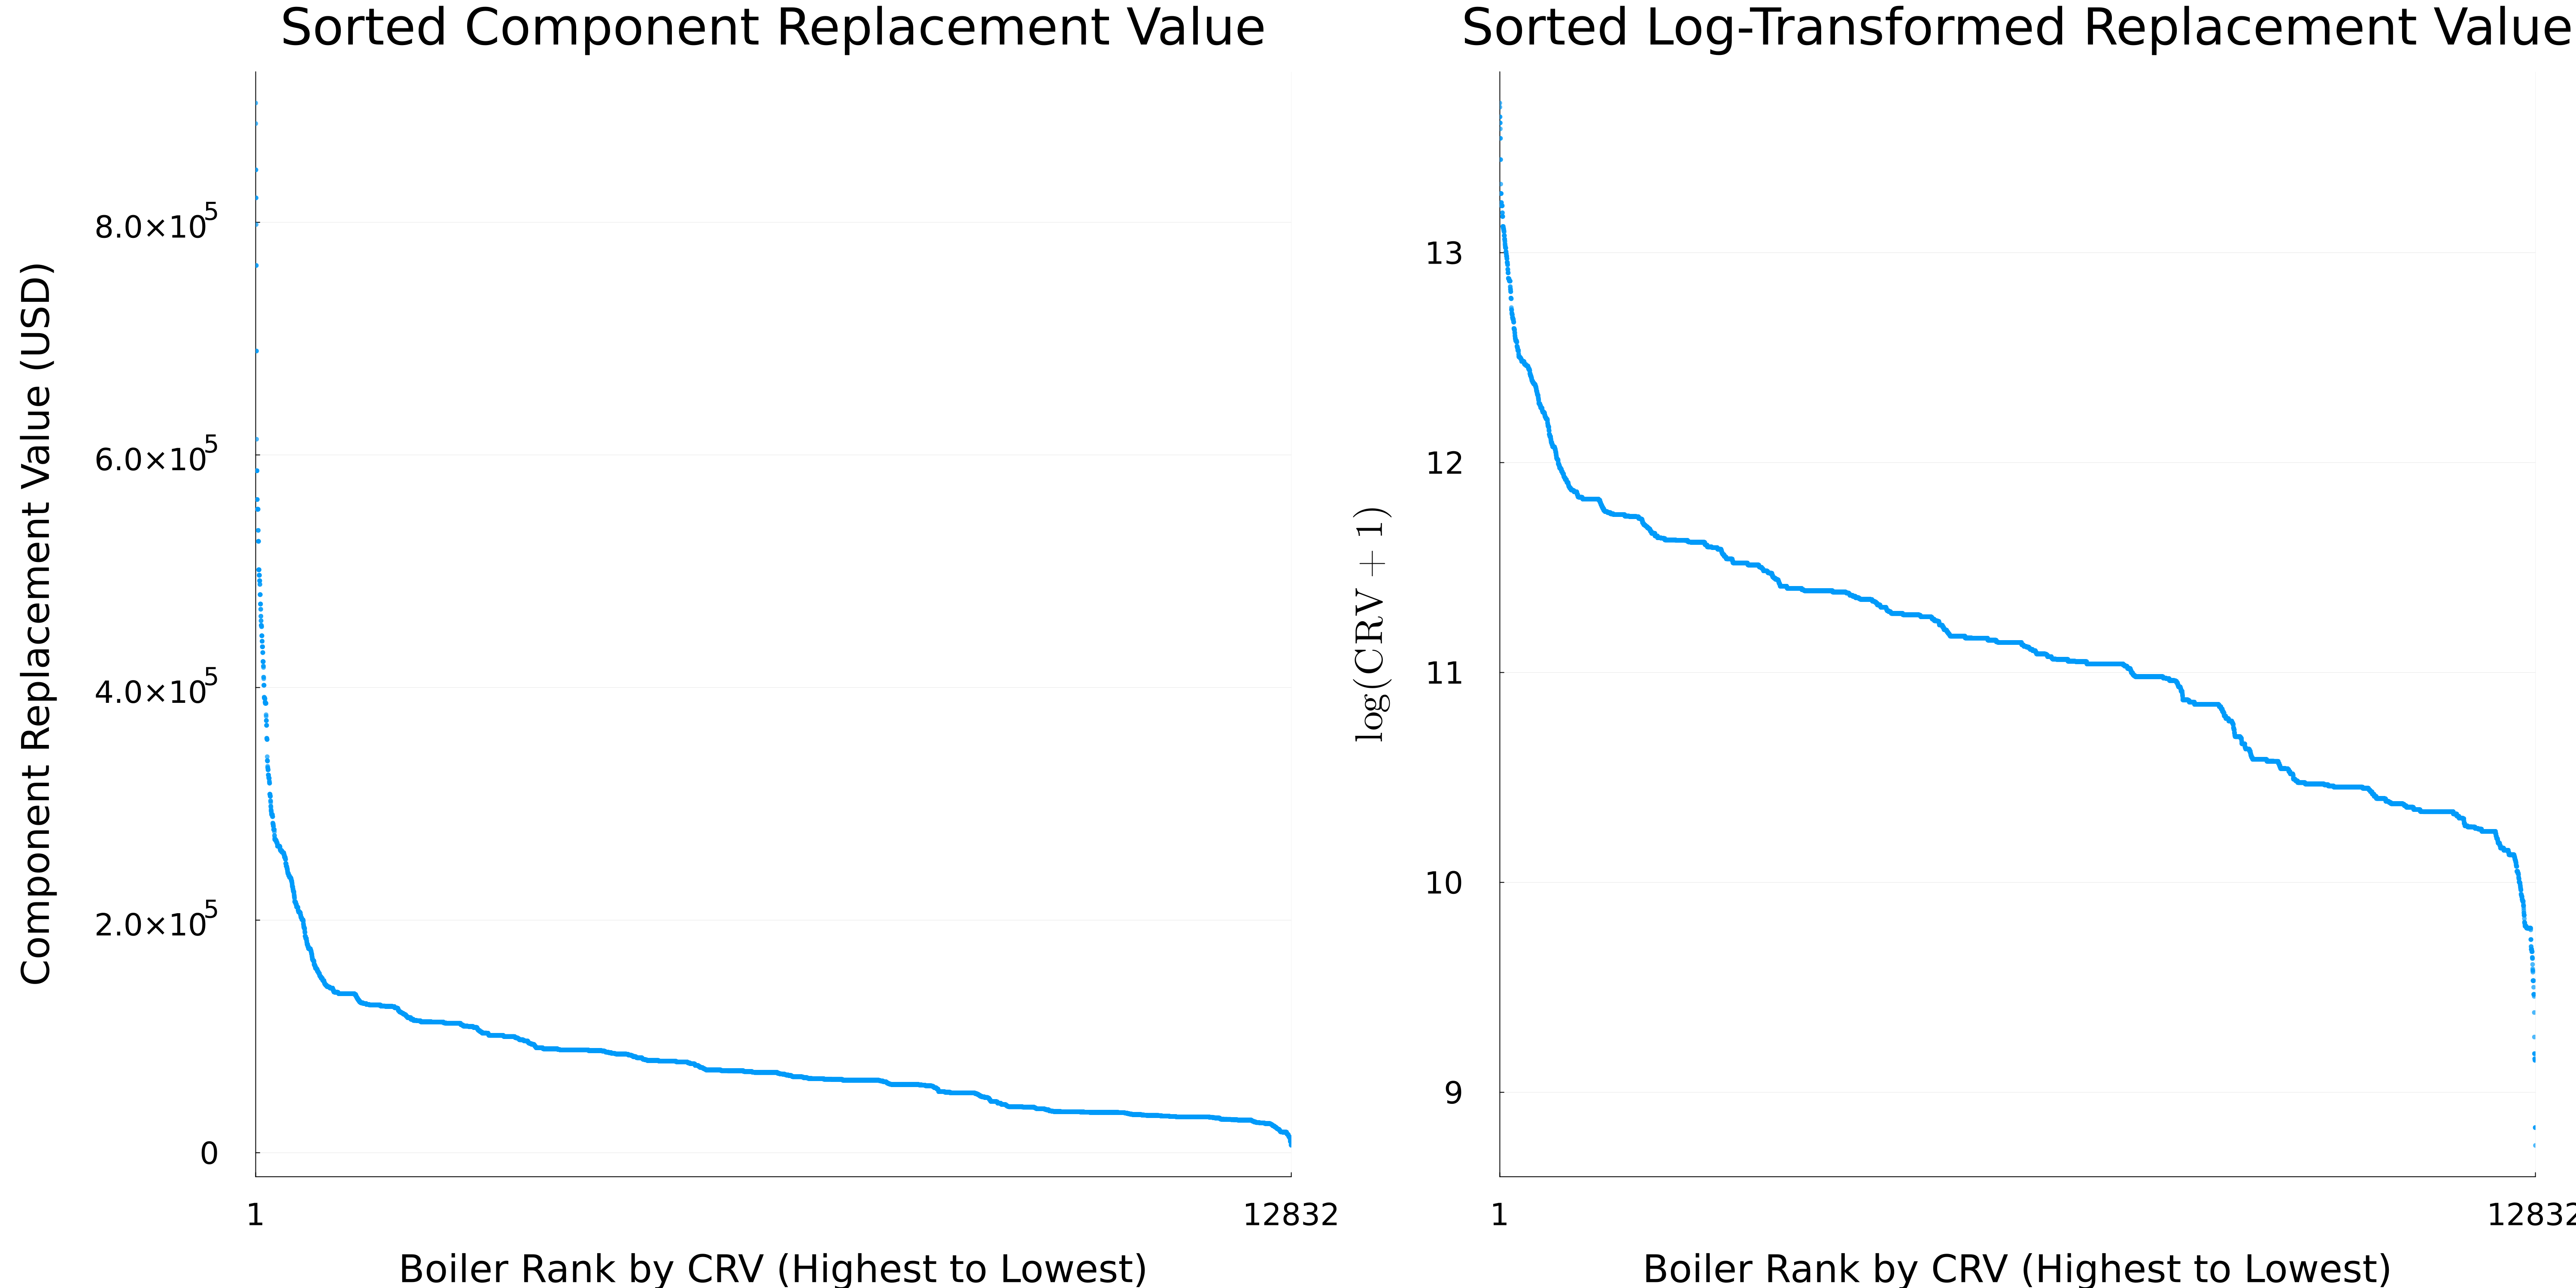
\includegraphics[width=1\linewidth]{log_crv_scatter.png}
\caption{Conversion of CRV to LogCRV}
\label{fig:crv_log}
\end{figure}

\newpage

\subsection{Principal Component Analysis}

With data wrangling steps completed, a PCA is performed using NormlizedAge, EffectiveAge, RSL, PredictedCI, Recency, PrevScore, PrevAssessed, NormalizedAssetAge, LogCRV, Year, MonthSin, MonthCos, and Climate columns of the cleaned dataset.  The first step of the PCA includes normalizing and standardizing the dataset (centering on mean, dividing by standard deviation). The SVD is generated and the Figure \ref{fig:pca_init} shows the initial explained variance by principal component. PC 1 has a notable dominance of 34\% of the explained variance. Upon inspection of PC 1, it was observed that all similarly derived lifecycle parameters (NormalizedAge, RSL, PredictedCI, and EffectiveAge) have roughly equal absolute values of ~.49 and seem to be relatively redundant. A new version is run choosing a single one of the lifecycle parameters, RSL is chosen by the rational that it is usually the easiest most people to understand by an interpretability standpoint. The resulting analysis produces a much smoother decline in explained variance across the PCs which can be seen in Figure \ref{fig:pca_reduced}. Of note, another version was run that included all lifecycle parameters divided by 4 to reduce overall influence, however the results were unremarkable and can be seen in Figure \ref{fig:scaled_lifecycle_pca}. All other insights if the PCA will refer to the reduced lifecycle iteration that was performed.

The loadings heatmap of the reduced parameter PCA shown in Figure \ref{fig:heatmap_reduced_pca} still shows the expected dominance of RSL in the first PC, but of note is a strong showing for Recency, Climate, and Month in PCs 2 and 3.  To search for potential predictability,  PC scores (Vt' x S) distributions are mapped back to assessed scores and color coded by "Green Region" (score >= 85) and "Not Green Region" (score < 85) and then plotted in histograms for each PC. Figure \ref{fig:score_dist_by_pc_reduced_pca} shows the results and unfortunately, no easily clear distinguishing characteristics jump out from the analysis. PC 1 which is dominated by RSL shows the most promise, but still has heavy overlap. Similar analysis is done for all 81 pairings of PC Scores color coded by region and plotted as scatter plots x vs y; the result was pretty mess of green and orange with no definitive separation of clusters. The resulting mega plot is omitted from this document, but be found in the repository under figures/pc\_vs\_pc\_score\_scatter.png.

\begin{figure}
\centering
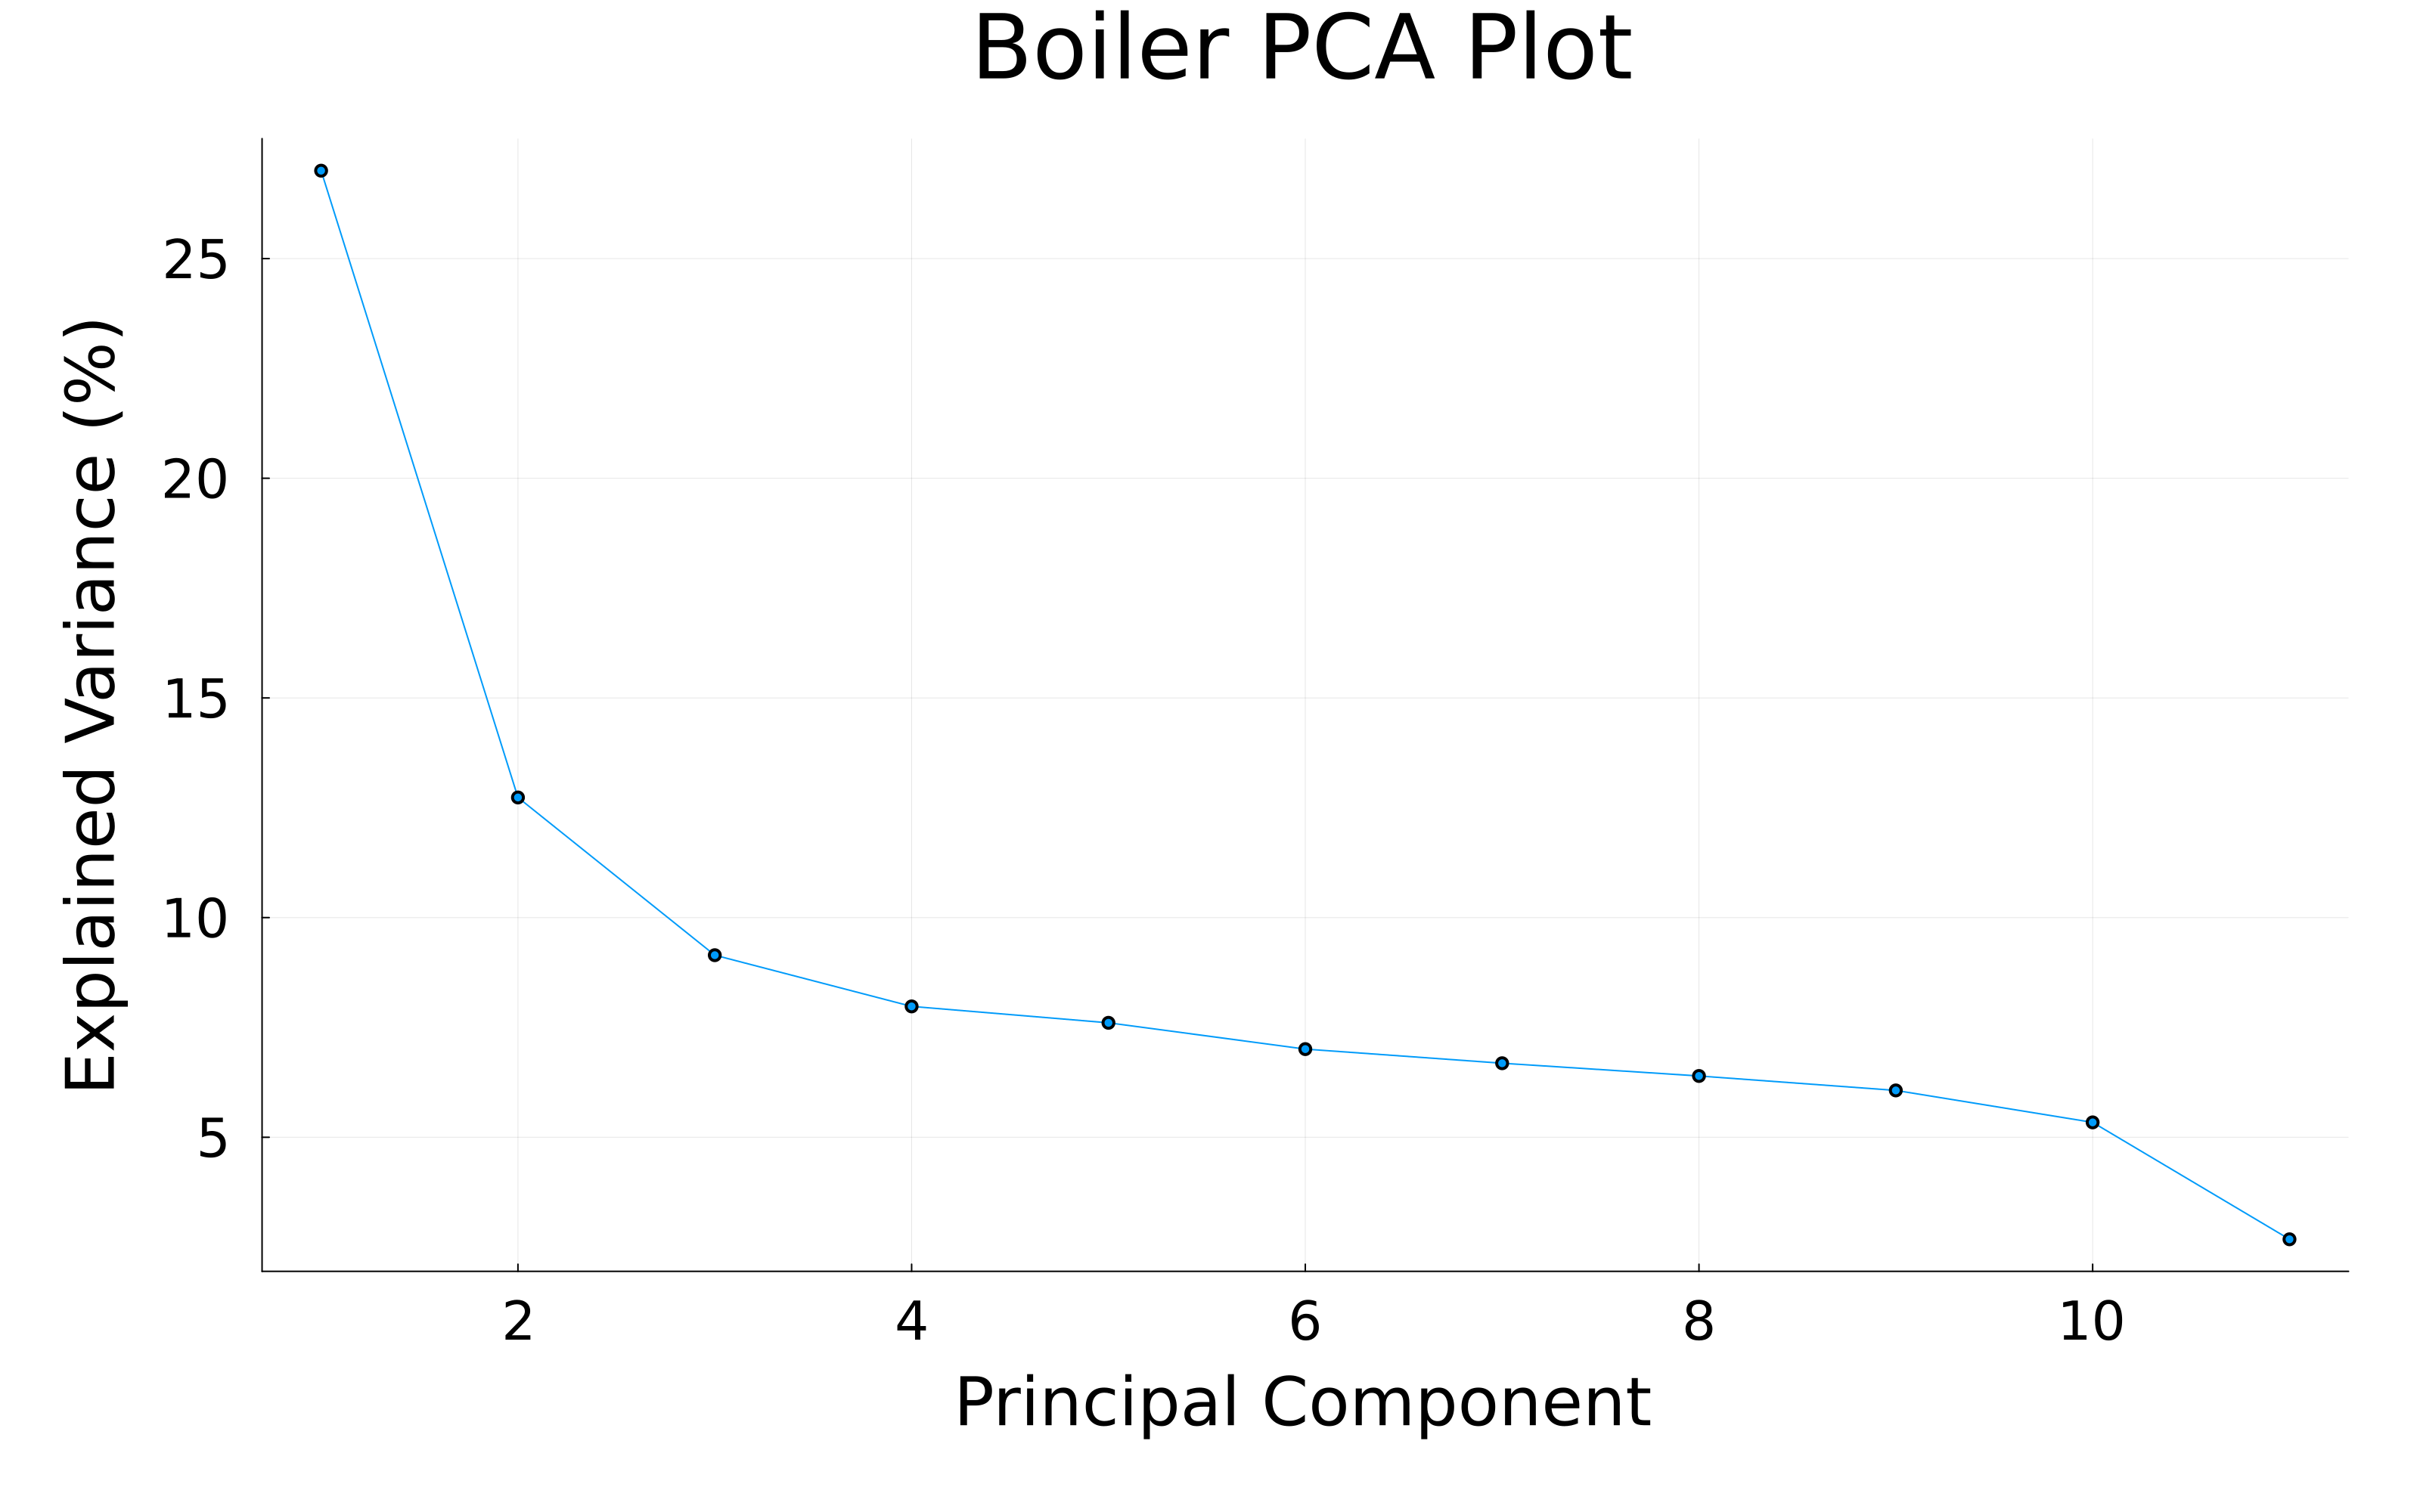
\includegraphics[width=1\linewidth]{pca_plot_initial.png}
\caption{Initial PCA Variance}
\label{fig:pca_init}
\end{figure}

\begin{figure}
\centering
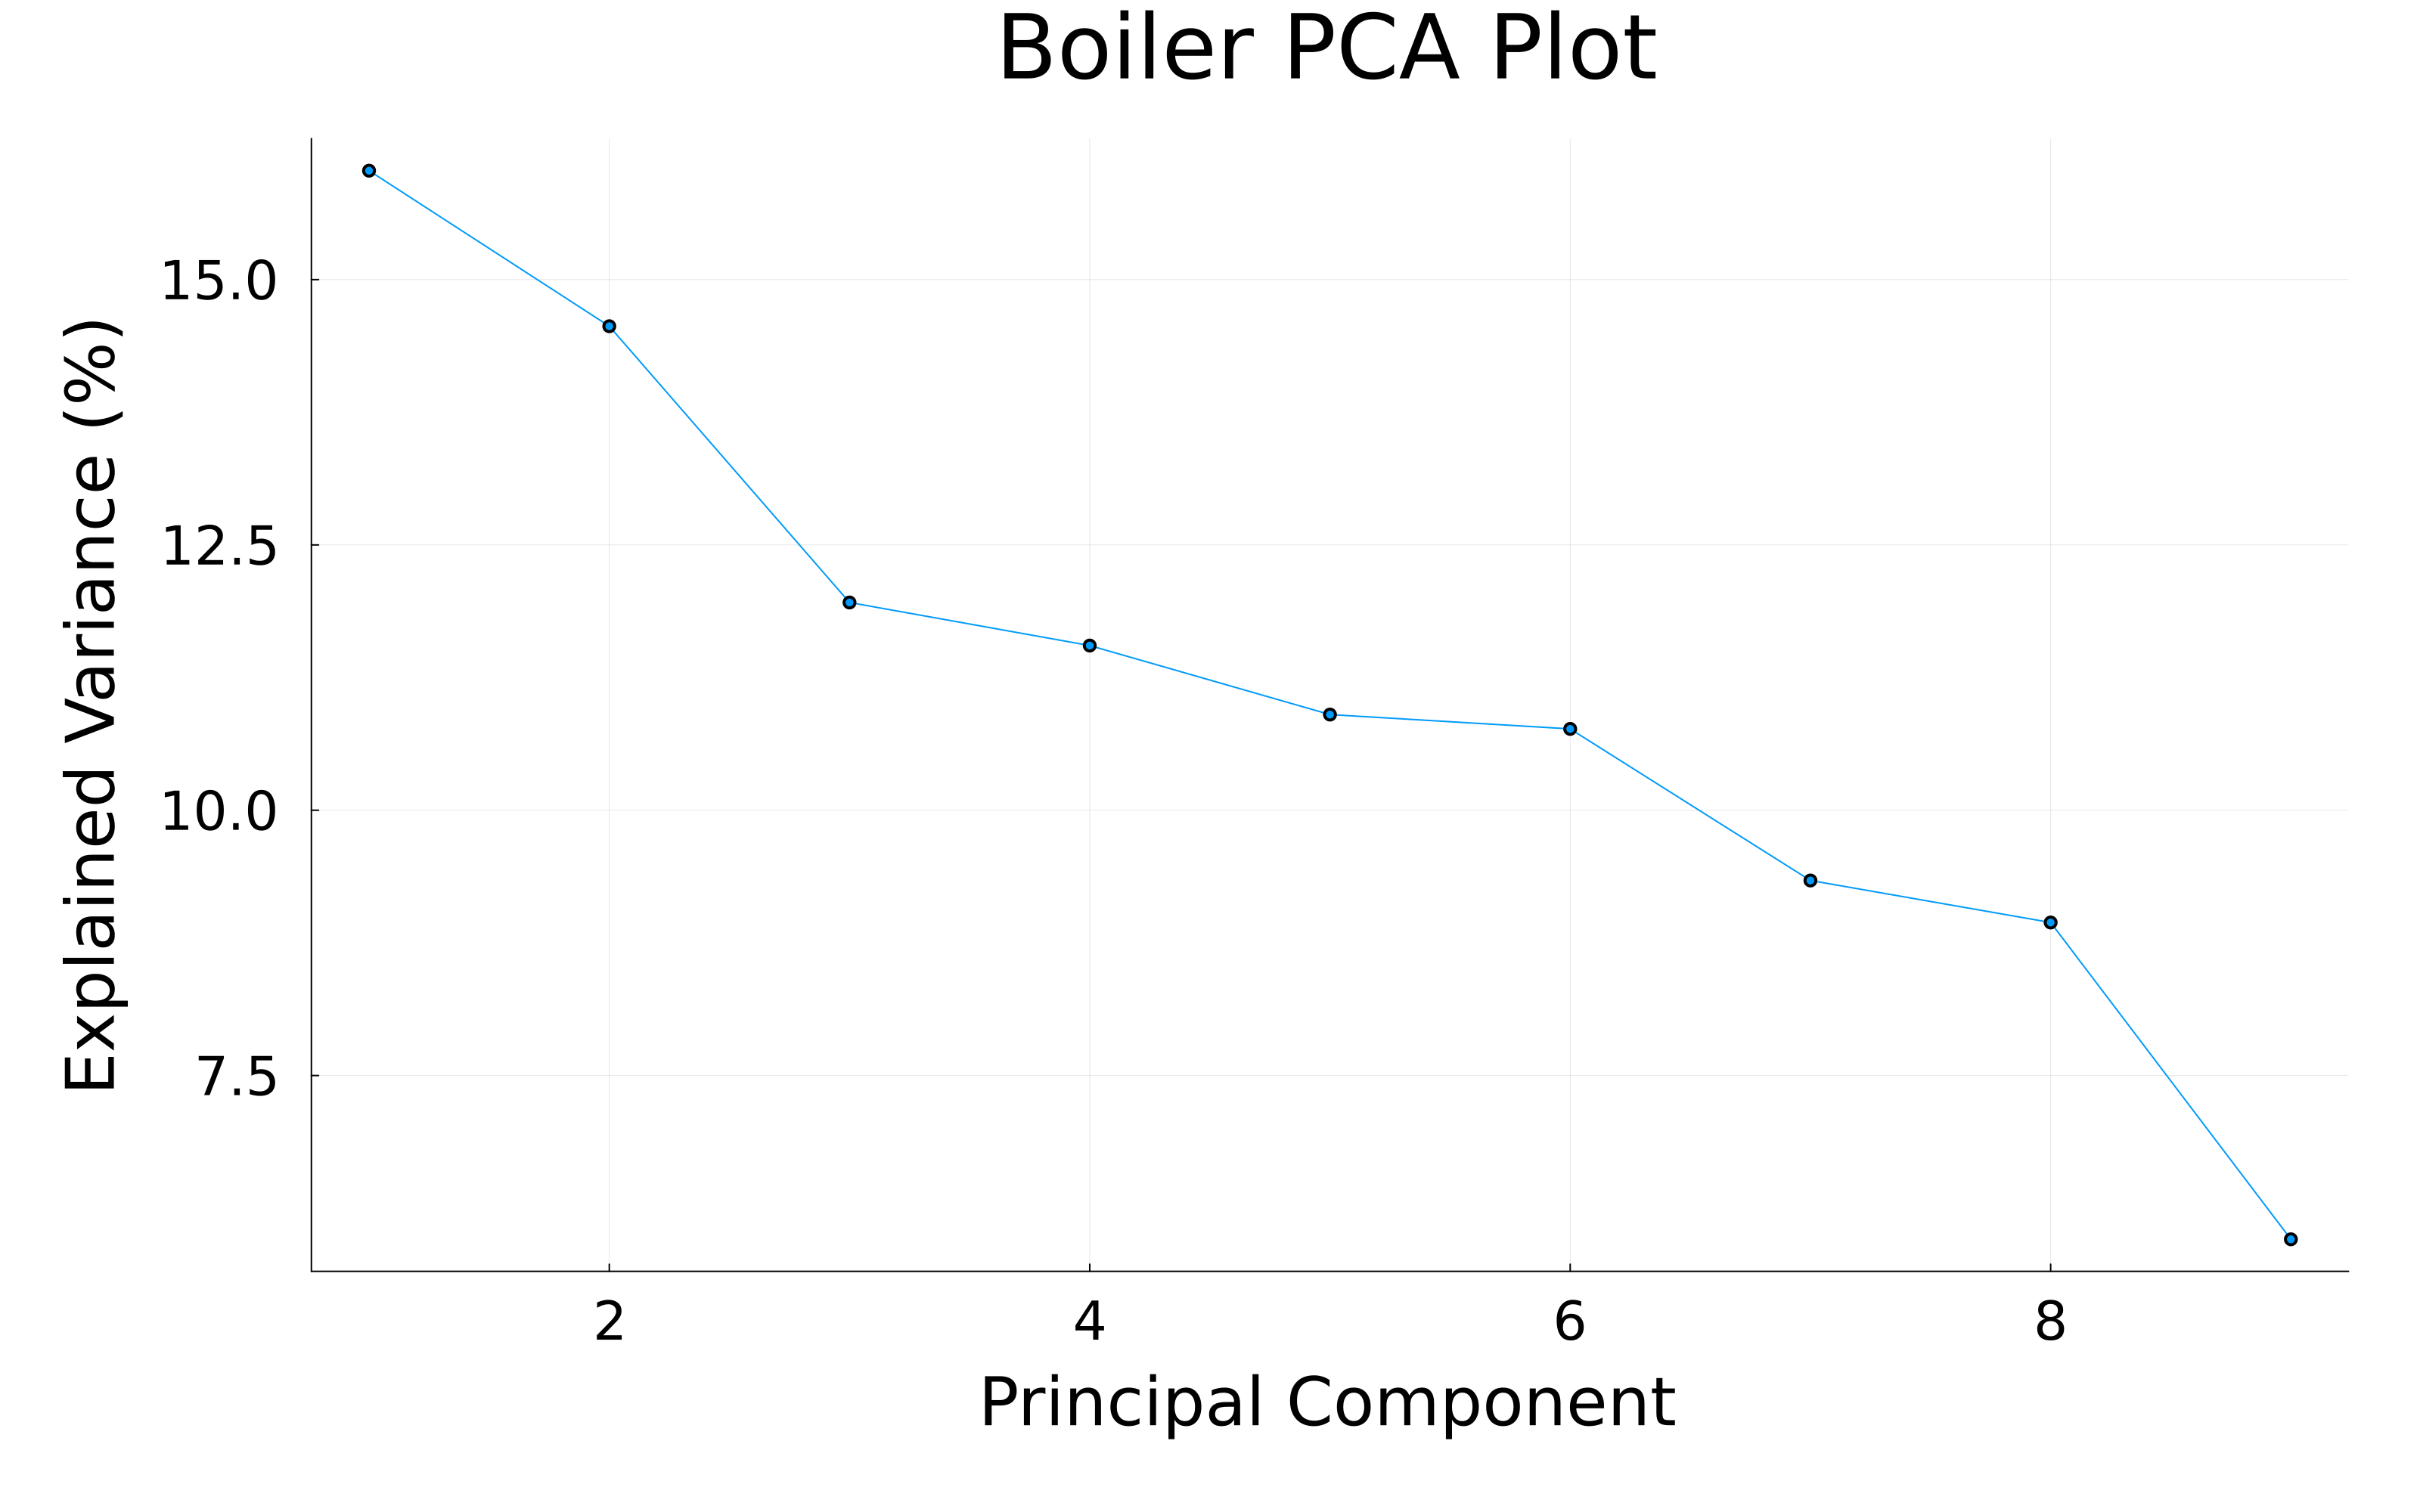
\includegraphics[width=1\linewidth]{pca_plot_reduced.png}
\caption{Reduced Parameter PCA Variance}
\label{fig:pca_reduced}
\end{figure}

\begin{figure}
\centering
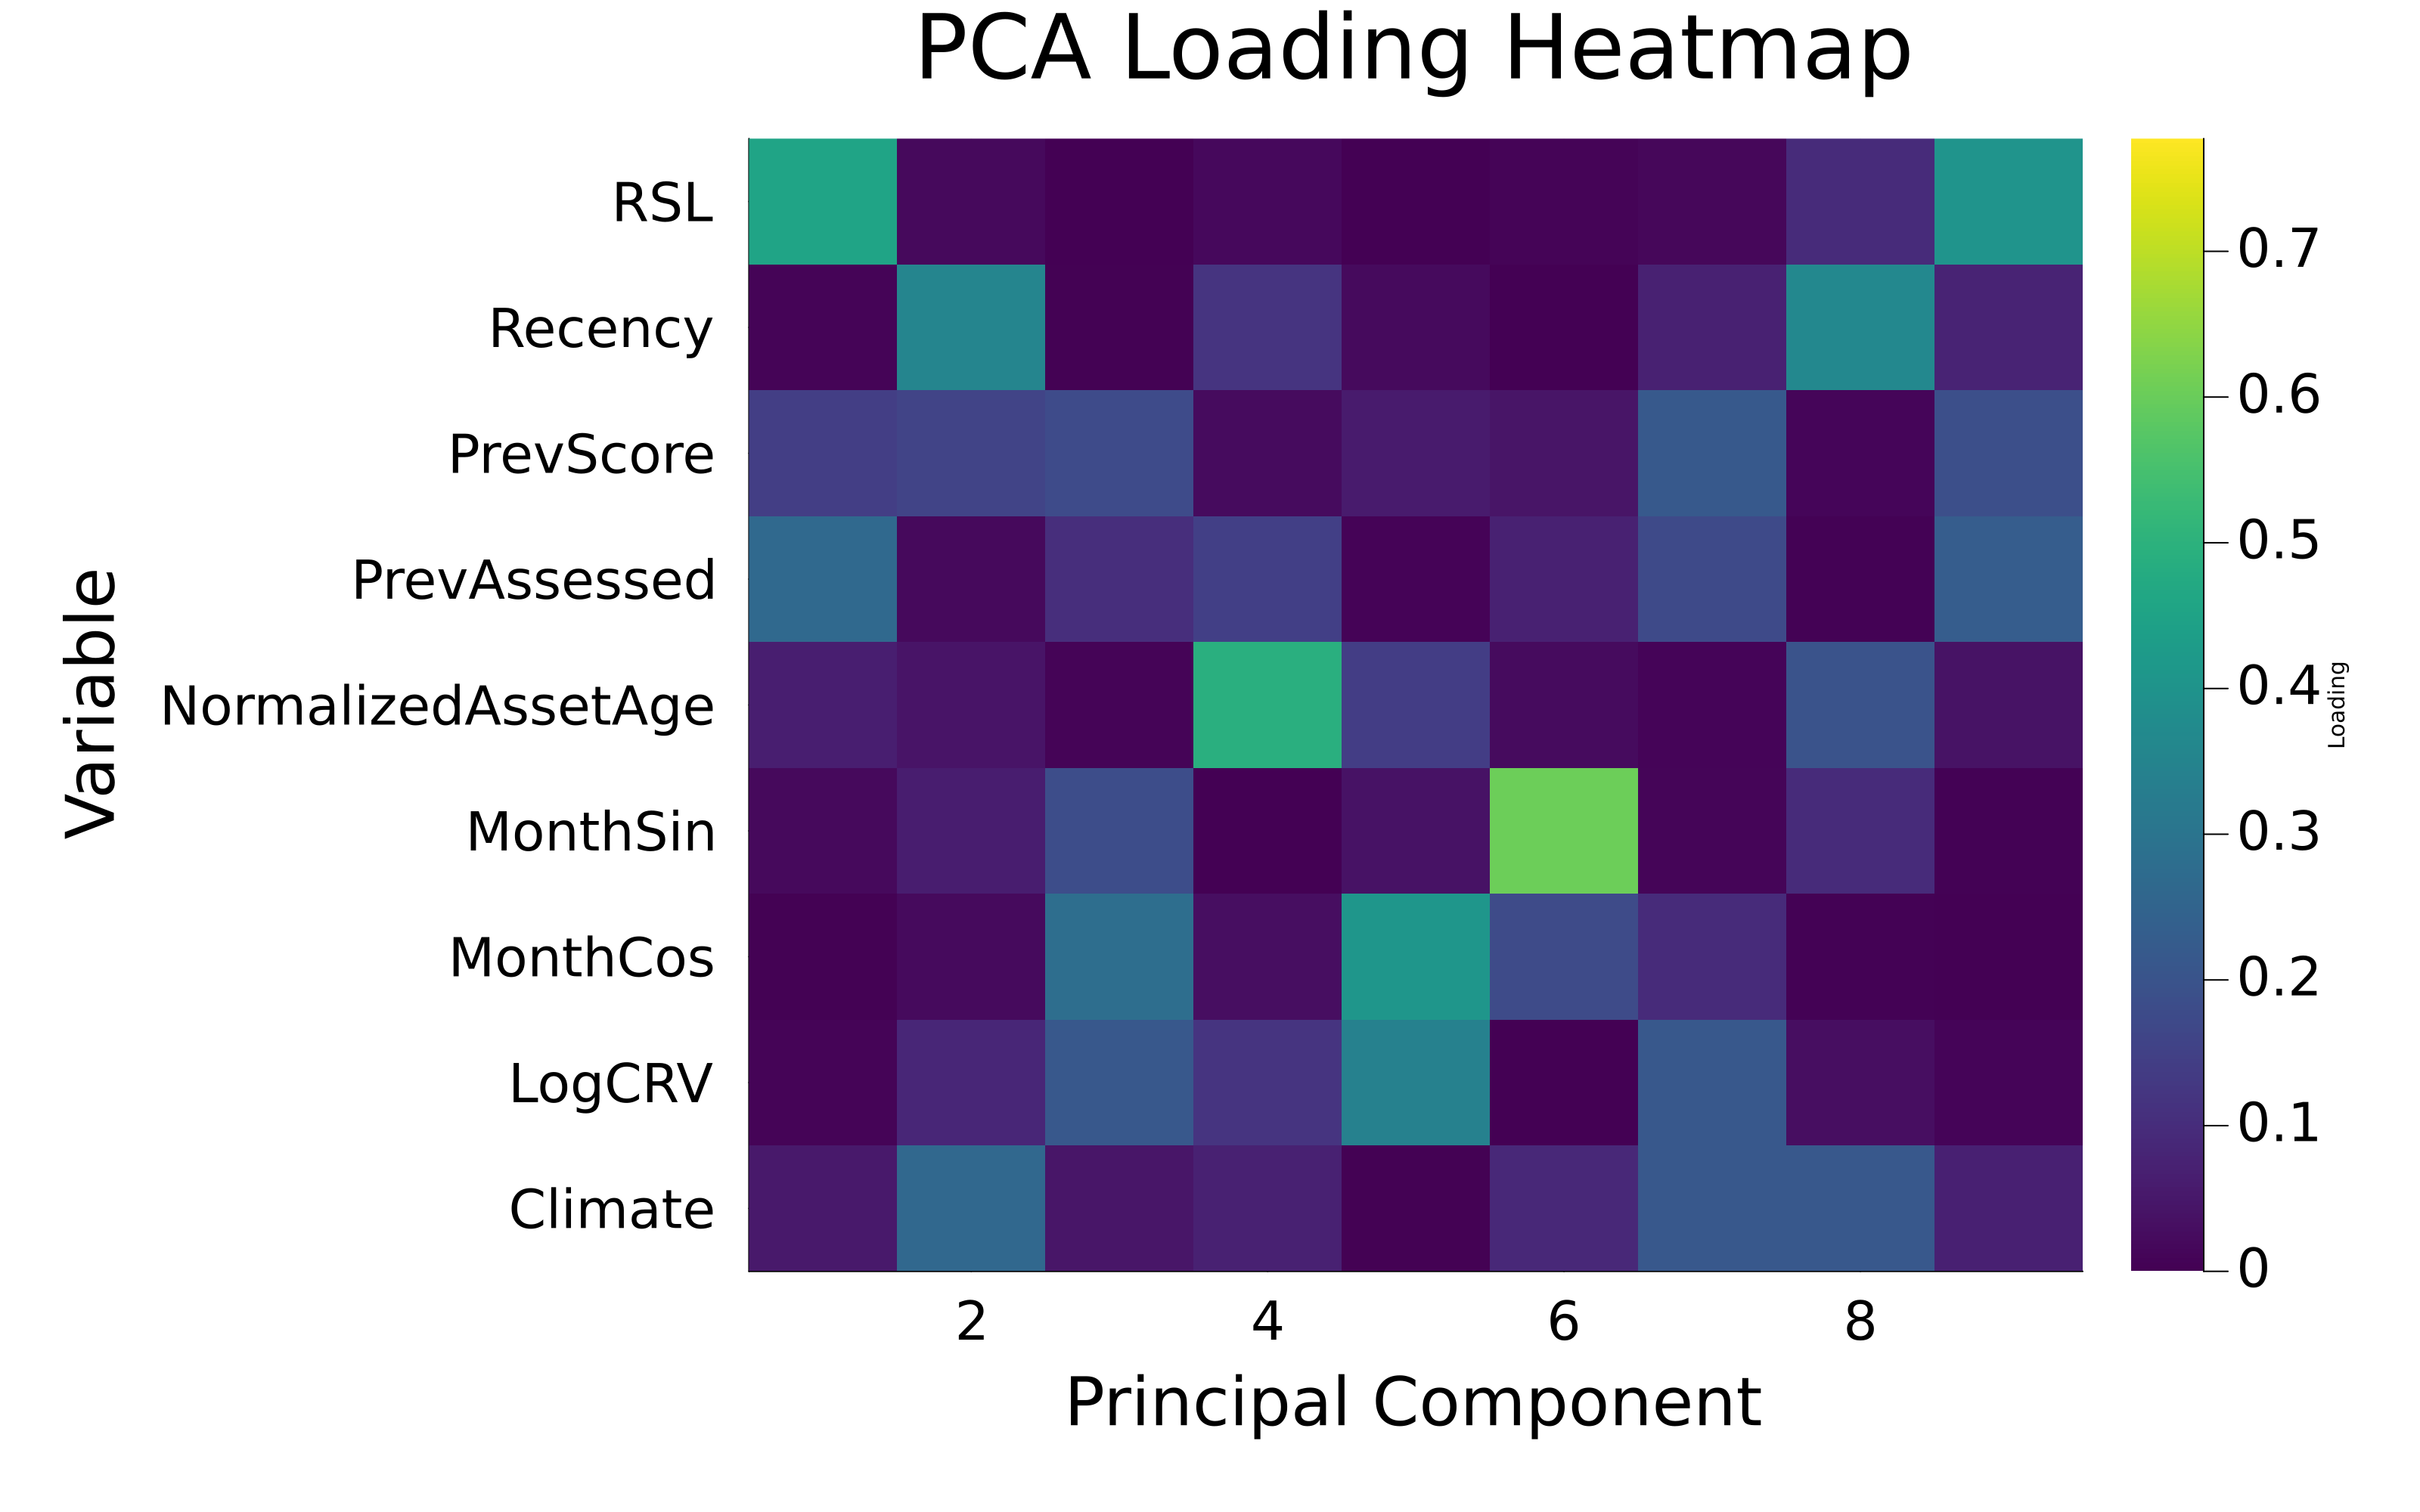
\includegraphics[width=1\linewidth]{loadings_heatmap_reduced_pca.png}
\caption{Loadings Heatmap for Reduced Parameter PCA}
\label{fig:heatmap_reduced_pca}
\end{figure}

\begin{figure}
\centering
\includegraphics[width=1\linewidth]{pc_vs_score_hists.png}f
\caption{Score Distributions by PC for Reduced Parameter PCA}
\label{fig:score_dist_by_pc_reduced_pca}
\end{figure}

\begin{figure}
\centering
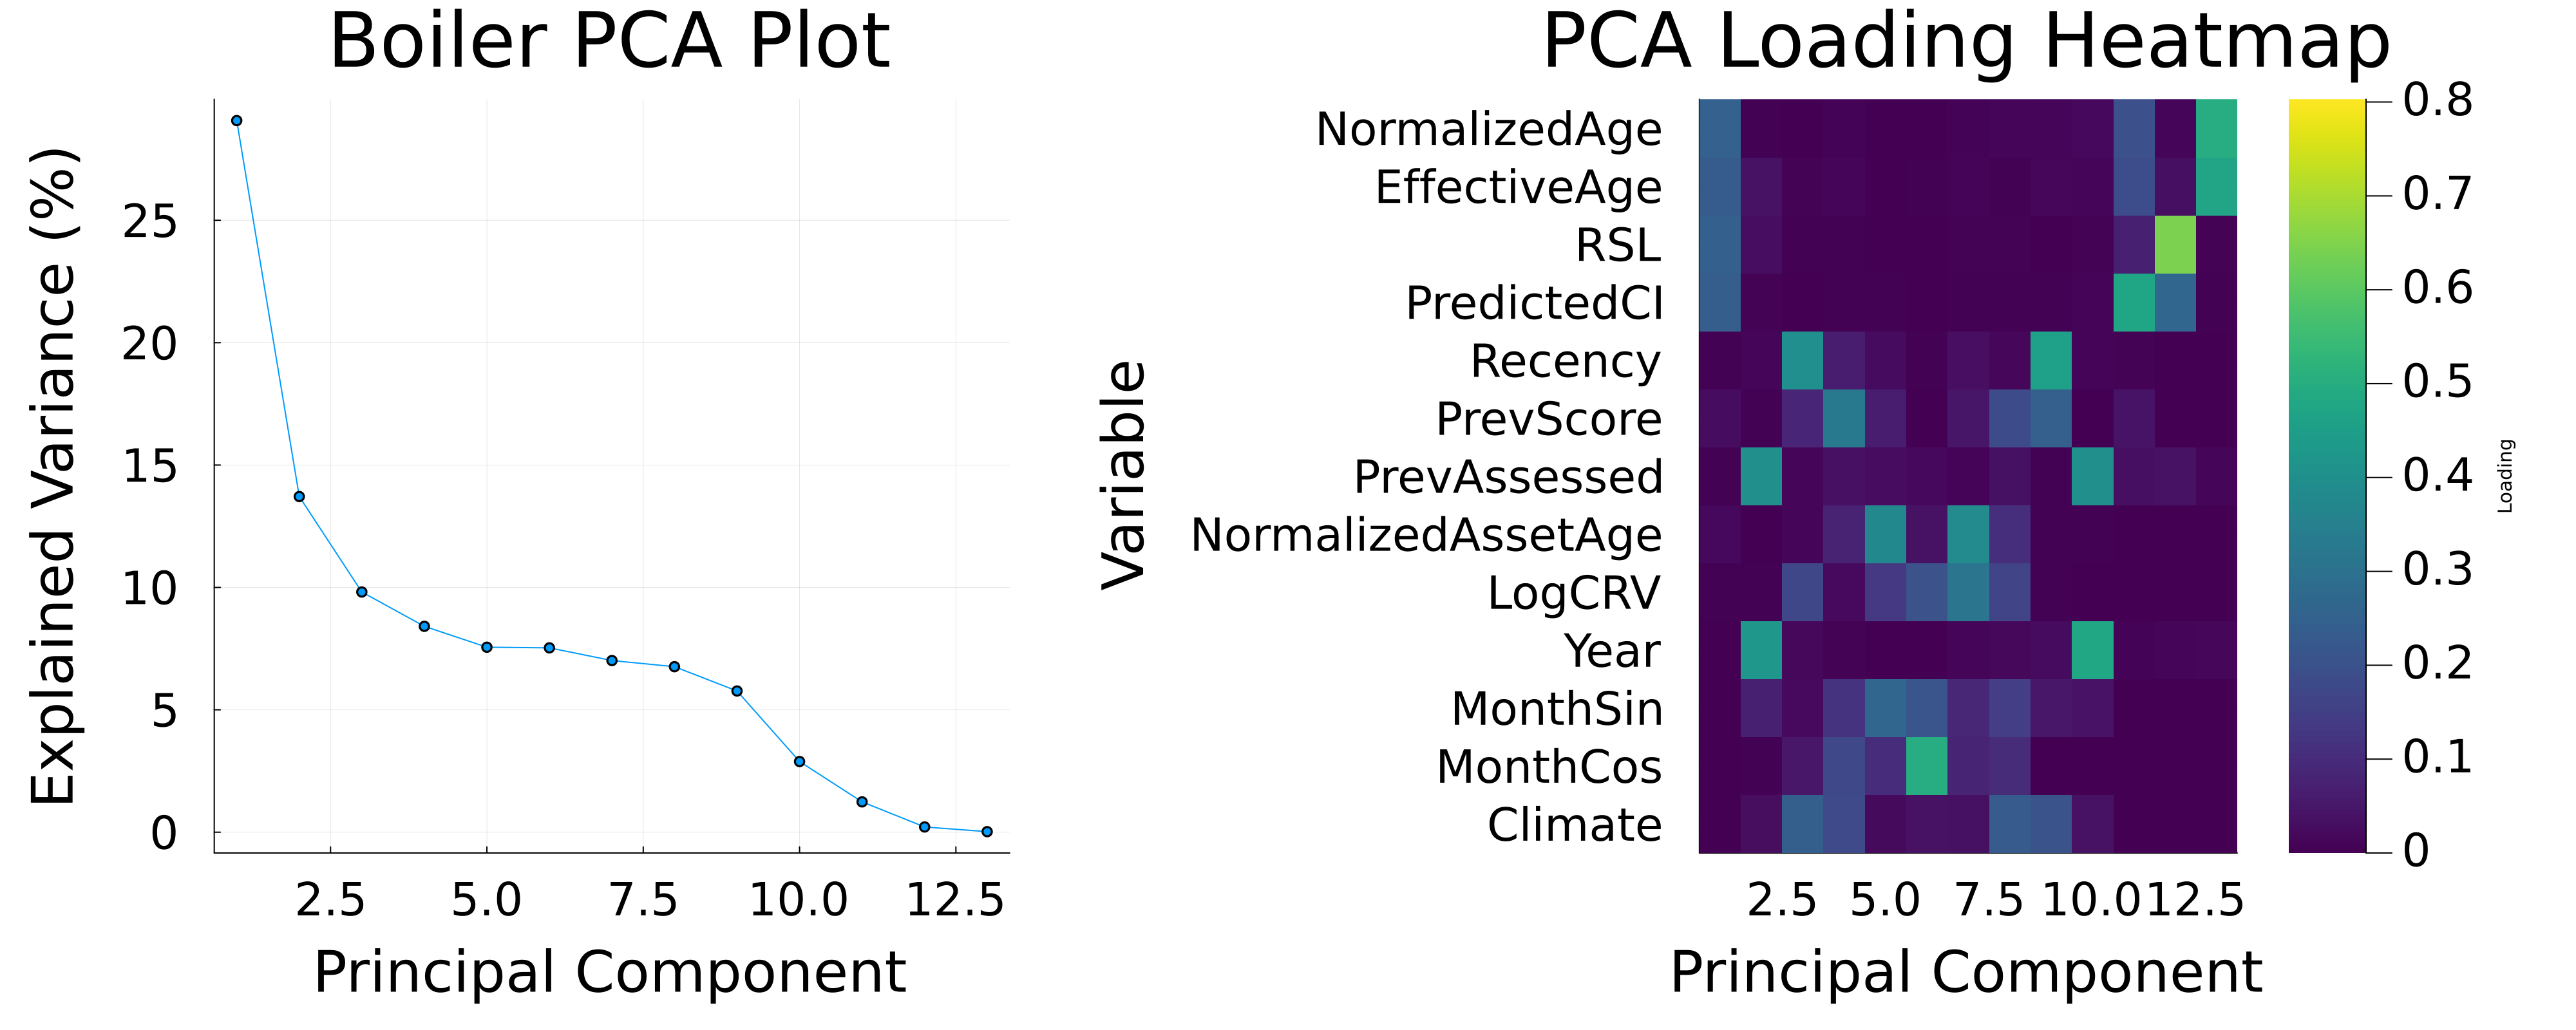
\includegraphics[width=1\linewidth]{scaled_lifecycle_pca.png}
\caption{Scaled Lifecycle PCA}
\label{fig:scaled_lifecycle_pca}
\end{figure}

\subsection{Additional Data Insights}
% Julian

\subsection{Regression Analysis}
% Juliana

\newpage

\begin{table}
\caption{Assessment Observation Data}
\label{table:assembly}
\centering
\small
\renewcommand{\arraystretch}{1.25}
\begin{tabular}{l l p{3.2in}}
\hline\hline
\multicolumn{1}{c}{Column} &
\multicolumn{1}{c}{Type (Units)} &
\multicolumn{1}{c}{Description} \\
\hline
Id & Int & Unique identifier for the observed component. Components can have multiple observations.\\
Spec & Int & Unique identifier for the specification of the component. This represents the specific type of inventory being assessed (i.e. 2 HP Pump, 400 gallon AST, etc.) \\
MEC & Int & Unique identifier for the Material Equipment Category. A less specific reference to the type of object being assessed (i.e. Pump, AST, Gas Boiler, etc.) \\
System & Int & Unique identifier for a very generic classification of the component (i.e. HVAC Equipment, Exterior Shell, Plumbing, etc.) \\
DesignLife & Int (Years) & Designed lifespan in years of the component. \\
Qty & Float (UOM) & Quantity of the component. Units defined by UOM. \\
UOM & String & Unit of Measure of the component Qty. \\
NormalizedAge & Float & Equal to $\text{ComponentAge} / \text{DesignLife}$. \\
EffectiveAge & Float & The curve adjusted age of the component at the time of assessment \\
RSL & Float & The adjusted remaining service life of the component equal to $\text{DesignLife} - \text{EffectiveAge}$ \\
Recency & Int (Years) & Number of years since the last assessment. Is empty if the component has not been assessed before. \\
PredictedCI & Float & Predicted Condition Index by the knowledge-based deterioration model at the time of the observation. Calculated using SMS Weibull Model. \\
Score & Float & Expert assessor's assigned condition rating. \\
CRV & Int (Dollars) & Component Replacement Value (i.e. Cost to replace the component) \\
Year & Int & Calendar year of the assessment. \\
Month & Int & Calendar month of the assessment. \\
Climate & Int & Department of Energy (DOE) based Climate Zones. \\
Fac & Int & Unique identifier for the type/purpose of the component's parent asset. \\
AssetAge & Int (Years) & Age in years of the component's parent asset. \\
AssetDesignLife & Int (Years) & Designed lifespan in years of the component's parent asset. \\
PrevScore & Float & Previous assessment score. Is empty if the component has not assessed before. \\
\hline
\multicolumn{3}{l}{$\ast$ System->MEC->Spec form a data hierarchy similar to a WBS like classification structure.} \\
\multicolumn{3}{l}{$\ast$ Data has been obfuscated, replacing readable definitions with numbers.} \\
\hline\hline
\end{tabular}
\normalsize
\end{table}

\begin{table}
\caption{Example Assessment Scoring Criteria based on USACE Guidance.}
\label{table:AssessmentScores}
\centering
\small
\renewcommand{\arraystretch}{1.25}
\begin{tabular}{l r p{3.5in}}
\hline\hline
\multicolumn{1}{c}{Rating} &
\multicolumn{1}{c}{CI Value} &
\multicolumn{1}{c}{Rating Definition} \\
\hline
Green (+) &
100 &
Entire component is free of observable distresses. Like-new condition. \\

Green &
95 &
No serviceability or reliability reduction. Slight degradation but noncritical. No work other than routine maintenance is required. \\

Green ($-$) &
88 &
Slight or no serviceability or reliability reduction. Some noticeable degradation is present but remains noncritical. No work other than routine maintenance is required. \\

Amber (+) &
79 &
Serviceability or reliability is degraded but remains adequate. Moderate deterioration is present but remains noncritical. Minor repairs are needed. \\

Amber &
68 &
Serviceability or reliability is noticeably impaired. Moderate deterioration or damage requires corrective repairs. \\

Amber ($-$) &
60 &
Significant serviceability or reliability loss. Significant degradation or damage requires major rehabilitation or overhaul. \\

Red (+) &
50 &
Significant serviceability or reliability loss. Repairs are not feasible, and replacement is needed. \\

Red &
25 &
Severe serviceability or reliability reduction may result in loss of use or safety. Immediate replacement is warranted. \\

Red ($-$) &
10 &
Complete degradation and loss of serviceability. May result in damage to surrounding components. Replace immediately. \\
\hline\hline
\end{tabular}
\normalsize
\end{table}

\newpage

\label{section:references}
\bibliography{./references.bib}
%
\end{document}
